\documentclass[11pt,twoside]{article}
\usepackage[preprint]{jmlr2e}
\usepackage{color}
\usepackage{fancyhdr}
\usepackage{amsfonts,epsfig,graphicx}
\usepackage{afterpage}
\usepackage{amsmath,amssymb} 
% \usepackage{fullpage}
\usepackage{epsf} 
\usepackage{graphics} 
\usepackage{amsfonts,amsmath}
% \usepackage[sort,numbers]{natbib} 
\usepackage{psfrag,xspace}
\usepackage{color,etoolbox}

\setlength{\textwidth}{\paperwidth}
\addtolength{\textwidth}{-6cm}
\setlength{\textheight}{\paperheight}
\addtolength{\textheight}{-4cm}
\addtolength{\textheight}{-1.1\headheight}
\addtolength{\textheight}{-\headsep}
\addtolength{\textheight}{-\footskip}
\setlength{\oddsidemargin}{0.5cm}
\setlength{\evensidemargin}{0.5cm}
\renewcommand{\floatpagefraction}{.8}%

\usepackage[utf8]{inputenc} % allow utf-8 input
\usepackage[T1]{fontenc}    % use 8-bit T1 fonts
\usepackage{hyperref}       % hyperlinks
\usepackage{url}            % simple URL typesetting
\usepackage{booktabs}       % professional-quality tables
\usepackage{amsfonts}       % blackboard math symbols
\usepackage{nicefrac}       % compact symbols for 1/2, etc.
\usepackage{microtype}      % microtypography

\usepackage{microtype}
\usepackage{graphicx}
\usepackage{float}
\usepackage[export]{adjustbox}
\usepackage{subcaption}
\usepackage{booktabs}
\usepackage{xcolor}
\usepackage{algorithm}
\usepackage{algorithmic}
\usepackage{enumerate}
\usepackage[shortlabels]{enumitem}
\usepackage{bm}
\usepackage{mathtools}

\DeclareFontFamily{U}{mathx}{\hyphenchar\font45}
\DeclareFontShape{U}{mathx}{m}{n}{<-> mathx10}{}
\DeclareSymbolFont{mathx}{U}{mathx}{m}{n}
\DeclareMathAccent{\wb}{0}{mathx}{"73}

\newcommand{\eqdist}{\ensuremath{\stackrel{d}{=}}}
\newcommand{\Graph}{\mathcal{G}}
\newcommand{\Reals}{\mathbb{R}}
\newcommand{\Identity}{\mathbb{I}}
\newcommand{\Xsetistiid}{\overset{\text{i.i.d}}{\sim}}
\newcommand{\convprob}{\overset{p}{\to}}
\newcommand{\convdist}{\overset{w}{\to}}
\newcommand{\Expect}[1]{\mathbb{E}\left[ #1 \right]}
\newcommand{\Risk}[2][P]{\mathcal{R}_{#1}\left[ #2 \right]}
\newcommand{\Prob}[1]{\mathbb{P}\left( #1 \right)}
\newcommand{\iset}{\mathbf{i}}
\newcommand{\jset}{\mathbf{j}}
\newcommand{\myexp}[1]{\exp \{ #1 \}}
\newcommand{\abs}[1]{\left \lvert #1 \right \rvert}
\newcommand{\restr}[2]{\ensuremath{\left.#1\right|_{#2}}}
\newcommand{\ext}[1]{\widetilde{#1}}
\newcommand{\set}[1]{\left\{#1\right\}}
\newcommand{\seq}[1]{\set{#1}_{n \in \N}}
\newcommand{\Xsetotp}[2]{\langle #1, #2 \rangle}
\newcommand{\floor}[1]{\left\lfloor #1 \right\rfloor}
\newcommand{\Var}{\mathrm{Var}}
\newcommand{\Cov}{\mathrm{Cov}}
\newcommand{\Xsetiam}{\mathrm{diam}}

\newcommand{\emC}{C_n}
\newcommand{\emCpr}{C'_n}
\newcommand{\emCthick}{C^{\sigma}_n}
\newcommand{\emCprthick}{C'^{\sigma}_n}
\newcommand{\emS}{S^{\sigma}_n}
\newcommand{\estC}{\widehat{C}_n}
\newcommand{\hC}{\hat{C^{\sigma}_n}}
\newcommand{\spansp}{\mathrm{span}~}
\newcommand{\1}{\mathbf{1}}

\newcommand{\Linv}{L^{\Xsetagger}}
\DeclareMathOperator*{\argmin}{argmin}
\DeclareMathOperator*{\argmax}{argmax}

\newcommand{\emF}{\mathbb{F}_n}
\newcommand{\emG}{\mathbb{G}_n}
\newcommand{\emP}{\mathbb{P}_n}
\newcommand{\F}{\mathcal{F}}
\newcommand{\D}{\mathcal{D}}
\newcommand{\R}{\mathcal{R}}
\newcommand{\Rd}{\Reals^d}
\newcommand{\Nbb}{\mathbb{N}}

%%% Vectors
\newcommand{\thetast}{\theta^{\star}}
\newcommand{\betap}{\beta^{(p)}}
\newcommand{\betaq}{\beta^{(q)}}
\newcommand{\vardeltapq}{\varDelta^{(p,q)}}


%%% Matrices
\newcommand{\X}{X} % no bold
\newcommand{\Y}{Y} % no bold
\newcommand{\Z}{Z} % no bold
\newcommand{\Lgrid}{L_{\grid}}
\newcommand{\Xsetgrid}{D_{\grid}}
\newcommand{\Linvgrid}{L_{\grid}^{\Xsetagger}}
\newcommand{\Lap}{{\bf L}}
\newcommand{\NLap}{{\bf N}}
\newcommand{\PLap}{{\bf P}}

%%% Sets and classes
\newcommand{\Xset}{\mathcal{X}}
\newcommand{\Sset}{\mathcal{S}}
\newcommand{\Hclass}{\mathcal{H}}
\newcommand{\Pclass}{\mathcal{P}}
\newcommand{\Leb}{L}
\newcommand{\mc}[1]{\mathcal{#1}}

%%% Distributions and related quantities
\newcommand{\Pbb}{\mathbb{P}}
\newcommand{\Ebb}{\mathbb{E}}
\newcommand{\Qbb}{\mathbb{Q}}
\newcommand{\Ibb}{\mathbb{I}}

%%% Operators
\newcommand{\Tadj}{T^{\star}}
\newcommand{\Xsetive}{\mathrm{div}}
\newcommand{\Xsetif}{\mathop{}\!\mathrm{d}}
\newcommand{\gradient}{\mathcal{D}}
\newcommand{\Hessian}{\mathcal{D}^2}
\newcommand{\dotp}[2]{\langle #1, #2 \rangle}
\newcommand{\Dotp}[2]{\Bigl\langle #1, #2 \Bigr\rangle}

%%% Misc
\newcommand{\grid}{\mathrm{grid}}
\newcommand{\critr}{R_n}
\newcommand{\Xsetx}{\,dx}
\newcommand{\Xsety}{\,dy}
\newcommand{\Xsetr}{\,dr}
\newcommand{\Xsetxpr}{\,dx'}
\newcommand{\Xsetypr}{\,dy'}
\newcommand{\wt}[1]{\widetilde{#1}}
\newcommand{\wh}[1]{\widehat{#1}}
\newcommand{\ol}[1]{\overline{#1}}
\newcommand{\spec}{\mathrm{spec}}
\newcommand{\LE}{\mathrm{LE}}
\newcommand{\LS}{\mathrm{LS}}
\newcommand{\OS}{\mathrm{OS}}
\newcommand{\PLS}{\mathrm{PLS}}
\newcommand{\dist}{\mathrm{dist}}
\newcommand{\vol}{\mathrm{vol}}
\newcommand{\cut}{\mathrm{cut}}

%%% Order of magnitude
\newcommand{\soom}{\sim}

\ShortHeadings{Local Spectral Density Clustering}{Green, Balakrishnan and Tibshirani}
\firstpageno{1}

%%%%%%%%%%%%%%%%%%%%%%%%%%%%%%%%%%%%%%%%%%%%%%%%%%%%%%%%%%%%%%%%%%%5

\begin{document}
	
\title{\textcolor{red}{The Geometry of Local Spectral Clustering}}

\author{\name Alden Green \email ajgreen@stat.cmu.edu \\
	\addr Department of Statistics and Data Science\\
	Carnegie Mellon University\\
	Pittsburgh, PA 15213
	\AND
	\name Sivaraman Balakrishnan \email sbalakri@stat.cmu.edu \\
	\addr Department of Statistics and Data Science\\
	Carnegie Mellon University\\
	Pittsburgh, PA 15213
	\AND
	Ryan J. Tibshirani \email ryantibs@stat.cmu.edu \\
	\addr Department of Statistics and Data Science\\
	Carnegie Mellon University\\
	Pittsburgh, PA 15213}

\maketitle

\begin{abstract}
	We analyze the Personalized PageRank (PPR) algorithm, a local spectral method
	for clustering, which extracts clusters using locally-biased random walks around
	a given seed node.  In contrast to previous work, we adopt a classical
	statistical learning setup, where we obtain samples from an unknown non-parametric distribution, and aim to identify geometrically salient clusters.  We introduce a pair of population-level geometric functionals---the \emph{normalized cut} and \emph{conductance}, analogous to graph-based functionals of the same name---and prove that PPR, run on a neighborhood graph, recovers clusters with small population normalized cut and large population conductance. We apply our general theory to establish that PPR identifies connected regions of high density (density clusters) that satisfy a set of natural geometric conditions. We also show a converse result, that PPR can fail to recover
	geometrically poorly-conditioned density clusters, even asymptotically. Finally,
	we provide empirical support for our theory.
\end{abstract}

\begin{keywords}
	graphs, spectral clustering, density clustering, Personalized PageRank, unsupervised learning
\end{keywords}


\section{Introduction}
In this paper, we consider the problem of clustering: splitting a given data set
into groups that satisfy some notion of within-group similarity and
between-group difference.  Our particular focus is on spectral clustering
methods, a family of powerful nonparametric clustering algorithms. Roughly
speaking, a spectral algorithm first constructs a geometric graph $G$, where
vertices correspond to samples, and edges correspond to proximities between
samples. The algorithm then estimates a feature embedding based on (an
appropriate) Laplacian matrix of $G$, and applies a simple clustering technique
(like $k$-means clustering) in the embedded feature space.

When applied to geometric graphs built from a large number of samples, global
spectral clustering methods can be computationally cumbersome and insensitive to
the local geometry of the underlying distribution
\citep{leskovec2010,mahoney2012}.  This has led to increased interest in
\emph{local} spectral clustering algorithms, which leverage locally-biased
spectra computed using random walks around some user-specified seed node.  A
popular local clustering algorithm is the Personalized PageRank (PPR) algorithm,
first introduced by \citet{haveliwala2003}, and then further developed by
several others
\citep{spielman2011,spielman2014,andersen2006,mahoney2012,zhu2013}.  

Local spectral clustering techniques have been practically very successful
\citep{leskovec2010,andersen2012,gleich2012,mahoney2012,wu2012}, which has led
many authors to develop supporting theory
\citep{spielman2013,andersen2009,gharan2012,zhu2013} that gives worst-case
guarantees on traditional graph-theoretic notions of cluster quality (such as normalized cut and conductance). In contrast, in this paper we adopt a classical statistical viewpoint, and examine what the output of local clustering on a data set reveals about the underlying density $f$ of the samples. \textcolor{red}{(We establish conditions on $f$ under which PPR, when appropriately tuned and initialized inside a candidate cluster $\mc{C}$, will approximately recover this candidate cluster. We pay special attention to the case where $\mc{C}$ is a \emph{density cluster} of $f$---defined as a connected component of the upper level set $\{x \in \Rd : f(x) \geq \lambda\}$ for some $\lambda > 0$---and show precisely how PPR accounts for both geometry and density in estimating a cluster.)}\\

\textcolor{red}{Alden: In our original submission, the preceding paragraph ended with the following sentence:
\begin{quote}
	In particular, we examine the ability of
	PPR to recover \emph{density clusters} of $f$, defined as the connected
	components of the upper level set $\{x \in \Rd : f(x) \geq \lambda\}$ for some
	$\lambda > 0$ (an object of central interest in the statistical clustering
	literature, dating back to the work of \citet{hartigan1981}). 
\end{quote}
This sentence no longer accurately describes our paper, so I substituted the part in parentheses above.}\\

Before giving a more detailed overview of our main results, we review some of the aforementioned worst-case guarantees, formally define PPR on a neighborhood graph, and introduce the population-level functionals that govern the behavior of local clustering \textcolor{red}{(in our statistical context)}. 

\subsection{Review: worst-case guarantees for local spectral clustering}
As mentioned, to date most analysis of local clustering has focused on worst-case guarantees, defined with respect to functionals of an a priori fixed graph $G = (V,E)$.  For instance, \cite{andersen2006} analyze the normalized cut of the cluster estimate $\wh{C}$ output by PPR. For a set $C \subseteq V$ with complement $C^c = V \!\setminus\! C$, the \emph{cut} and \emph{volume} are respectively,
\begin{equation}
\label{eqn:cut_volume}
\cut(C;G) := \sum_{u \in C} \sum_{v \in C^c}
\1\{(u,v) \in E\},~~ \vol(C; G) := \sum_{u \in C}  \sum_{v \in V} \1\{(u,v) \in E\},
\end{equation}
and the \emph{normalized cut} of $C$ is
\begin{equation}
\label{eqn:normalized_cut}
\Phi(C; G) := \frac{\cut(C;G)}{\min \set{\vol(C; G), \vol(C^c; G)}}.
\end{equation} 
\cite{andersen2006} show that when PPR is appropriately seeded within a candidate cluster $C \subseteq V$, the normalized cut of the candidate cluster is upper bounded $\Phi(\wh{C};G) \lesssim \sqrt{\Phi(C;G)}$. \cite{zhu2013} build on this: they introduce a second functional, the \emph{conductance} $\Psi(G)$, defined as 
\begin{equation}
\label{eqn:conductance}
\Psi(G) := \min_{S \subseteq V} \Phi(S;G),
\end{equation}
and show that if $\Phi(C;G)$ is much smaller than $\Psi(G[C])^2$---where $G[C] = (C,E \cap (C \times C))$ is the subgraph of $G$ induced by $C$--- then (in addition to having a small normalized cut) the cluster estimate $\wh{C}$ approximately recovers $C$. Our own analysis will build on that of~\cite{zhu2013}, and we will give a more detailed summary of their results in Section~\ref{sec:ub_symmetric_set_difference}.
For now, we merely reiterate that the conclusions of \citep{andersen2006,zhu2013} cannot be straightforwardly applied to our statistical setting, where the input data are random samples $\{x_1,\ldots,x_n\}$ drawn from a distribution $\mathbb{P}$, the graph $G$ is a random geometric graph formed by the user, and the candidate cluster is a set $\mc{C} \subset \Rd$. 

\subsection{PPR on a neighborhood graph}

We now formally describe this setting, as well as the method we will study: PPR on a neighborhood graph. Let $X = \{x_1,\ldots, x_n\}$ be samples drawn i.i.d.\ from a distribution
$\Pbb$ on $\Rd$. We will assume throughout that $\Pbb$ has a density $f$ with respect to the Lebesgue measure on $\Rd$. For a radius $r > 0$, we define
$G_{n,r}=(V,E)$ to be the \emph{$r$-neighborhood graph} of $X$, an
unweighted, undirected graph with vertices $V=X$, and an edge $(x_i,x_j) \in
E$ if and only if $\|x_i - x_j\| \leq r$, where $\|\cdot\|$ is the
Euclidean norm. We denote by $A \in \Reals^{n \times n}$ the adjacency
matrix, with entries $A_{uv} = 1$ if $(u,v) \in E$ and $0$ otherwise.  We
also denote by $D$ the diagonal degree matrix, with entries $D_{uu} :=
\sum_{v \in V} A_{uv}$, and by $I{}$ the $n \times n$ identity matrix.

The PPR vector $p_v = p(v,\alpha;G_{n,r})$ is defined with respect to
a given seed node $v \in V$ and a teleportation parameter $\alpha \in [0,1]$, as the solution of the following linear system:
\begin{equation}
\label{eqn: ppr_vector}
p_v = \alpha e_{v} + (1 - \alpha) p_v W,
\end{equation}
where $W = (I + D^{-1}A)/2$ is the lazy random walk matrix over
$G_{n,r}$ and $e_{v}$ is the indicator vector for node $v$ (that has a 1 in
position $v$ and 0 elsewhere).  

Once $p_v$ is computed, the cluster estimate $\wh{C}$ is chosen by taking a particular sweep cut of $p_v$. For a given level $\beta > 0$, the \emph{$\beta$-sweep cut} of $p_v = (p_v(u))_{u \in V}$ is 
\begin{equation}
\label{eqn: sweep_cuts}
S_{\beta,v} := \set{u \in V: \frac{p_v(u)}{D_{uu}} > \beta}.
\end{equation}
To determine $\wh{C}$, one computes $S_{\beta,v}$ over all \smash{$\beta \in (L, U)$} (where the range $(L,U)$ is user-specified), and then outputs the cluster estimate
\smash{$\wh{C} = S_{\beta^*}$} with minimum normalized cut.  For concreteness,
the PPR algorithm is summarized in Algorithm~\ref{alg:ppr}.   

\begin{algorithm}
	\caption{PPR on a neighborhood graph}
	\label{alg:ppr}	
	{\bfseries Input:} data $X=\{x_1,\ldots,x_n\}$, radius $r > 0$, teleportation
	parameter $\alpha \in [0,1]$, seed $v \in X$, sweep cut range $(L,U)$. \\     
	{\bfseries Output:} cluster estimate $\wh{C} \subseteq V$.
	\begin{algorithmic}[1]
		\STATE Form the neighborhood graph $G_{n,r}$.
		\STATE Compute the PPR vector $p_v=p(v, \alpha; G_{n,r})$ as in
		\eqref{eqn: ppr_vector}.  
		\STATE For \smash{$\beta \in (L,U)$}, compute sweep cuts $S_{\beta}$ as in
		\eqref{eqn: sweep_cuts}. 
		\STATE Return the cluster \smash{$\wh{C} = S_{\beta^*}$}, where  
		$$
		\beta^* = \argmin_{\beta \in (L,U)}~ \Phi(S_{\beta}; G_{n,r}).
		$$
	\end{algorithmic}
\end{algorithm}


\subsection{Cluster estimation}
We need a metric to assess the accuracy with which $\wh{C}$ estimates the candidate cluster $\mc{C}$. One commonly used metric is the misclassification error, i.e. the size of the symmetric set difference
between $\wh{C}$ and the empirical cluster $\mc{C}[X] = \mc{C} \cap X$ \citep{korostelev1993,polonik1995,rigollet2009}. We
will consider a related metric, the volume of the symmetric set difference,
which weights misclassified points according to their degree in $G_{n,r}$. To keep things simple, for a given set $S \subseteq X$ we write $\vol_{n,r}(S) := \vol(S;G_{n,r})$. 
\begin{definition}
	\label{def:volume_symmetric_set_difference}
	For an estimator \smash{$\wh{C} \subseteq X$} and a set 
	$\mathcal{C} \subseteq \Rd$, their symmetric set difference is 
	\begin{equation*}
	\wh{C} \vartriangle \mathcal{C}[X] :=
	\bigl(\wh{C} \setminus \mathcal{C}[X]\bigr) \cup
	\bigl(\mathcal{C}[X] \setminus \wh{C}\bigr).
	\end{equation*}
	Furthermore, we denote the volume of the symmetric set difference by 
	$$
	\Delta(\wh{C}, \mathcal{C}[X]) := \vol_{n,r}(\wh{C} \vartriangle \mathcal{C}[X]). 
	$$
\end{definition}

\subsection{Population normalized cut and conductance}
As we will show, the volume of the symmetric set difference $\Delta(\wh{C},\mc{C}[X])$ is intrinsically related to two population-level functionals of $\mc{C}$, the normalized cut $\Phi_{\Pbb,r}(\mc{C})$ and conductance $\Psi_{\Pbb,r}(\mc{C})$, which we now define. Let the population-level \emph{cut} of $\mc{C}$ be the expectation (up to a rescaling) of $\cut_{n,r}(\mc{C}[X]) := \cut(\mc{C}[X]; G_{n,r})$,  and likewise let the population-level \emph{volume} of $\mc{C}$ be the expectation (up to a rescaling) of $\vol_{n,r}(\mc{C}[X]) = \vol(\mc{C}[X]; G_{n,r})$; i.e. let
\begin{equation*}
\mathrm{cut}_{\Pbb,r}(\mc{C}) := \int_{\mc{C}} \int_{\mc{C}^c} \1\{\|x - y\| \leq r\} \,d\Pbb(y) \,d\Pbb(x)~~ \mathrm{vol}_{\Pbb,r}(\mc{C}) := \int_{\mc{C}} \int_{\Rd} \1\{\|x - y\| \leq r\} \,d\Pbb(y) \,d\Pbb(x),
\end{equation*}
where $\mc{C}^c := \Rd \!\setminus\! \mc{C}$.
\begin{definition}[Population normalized cut]
	For a set $\mc{C} \subset \Rd$, distribution $\Pbb$ with density $f$, and radius $r > 0$, the \emph{population normalized cut} is
	\begin{equation}
	\label{eqn:population_normalized_cut}
	\Phi_{\Pbb,r}(\mc{C}) := \frac{\mathrm{cut}_{\Pbb,r}(\mc{C})}{\min\{\mathrm{vol}_{\Pbb,r}(\mc{C}), \mathrm{vol}_{\Pbb,r}(\mc{C}^c)\}}
	\end{equation}
\end{definition}

Let $\wt{\mathbb{P}}(\cdot) = \mathbb{P}(\cdot|x \in \mc{C})$ be the conditional distribution of $x$, i.e. the distribution with density function
\begin{equation*}
\wt{f}(x) :=
\begin{cases*}
\frac{1}{\mathbb{P}(\mc{C})} f(x),~~ & \textrm{if $x \in \mc{C}$} \\
0,~~ & \textrm{otherwise.}
\end{cases*}
\end{equation*}

\begin{definition}[Population conductance]
	For a set $\mc{C} \subset \Rd$, distribution $\Pbb$ with density $f$, and radius $r > 0$, the \emph{population conductance} is
	\begin{equation}
	\label{eqn:population_conductance}
	\Psi_{\mathbb{P},r}(\mc{C}) = \inf_{\mc{S} \subseteq \mc{C}} \Phi_{\wt{\Pbb},r}(\mc{S})
	\end{equation}
\end{definition}

It is quite natural that $\Phi_{\Pbb,r}(\mc{C})$ and $\Psi_{\Pbb,r}(\mc{C})$ should help quantify the role geometry plays in local spectral clustering. Indeed, by construction these functionals are quite obviously the population-level analogues of the empirical quantities $\Phi_{n,r}(\mc{C}[X]) := \Phi(\mc{C}[X];G_{n,r})$ and $\Psi_{n,r}(\mc{C}[X]) = \Psi(G_{n,r}\bigl[\mc{C}[X]\bigr])$, and as we have already mentioned, these empirical quantities in turn suffice to upper bound the volume of the symmetric set difference. For this reason, similar population level functionals are used by \citep{shi2009,schiebinger2015,garciatrillos19} in the analysis of \emph{global} spectral clustering in a statistical context. We will comment more on the relationship between these works and our own results in~\ref{subsec:related_work}.

\subsection{Summary of results}
A summary of our results (and an outline for this paper) is as follows.
\begin{itemize}
	\item In Section~\ref{sec:ub_symmetric_set_difference}, we show that the sample normalized cut $\Phi_{n,r}(\mc{C}[X])$ and conductance $\Psi_{n,r}(\mc{C}[X])$ are close to their population level counterparts $\Phi_{\Pbb,r}(\mc{C})$ and $\Psi_{\Pbb,r}(\mc{C})$. As a consequence, we find that $\Delta(\wh{C},\mc{C}[X])$ is small whenever $\Phi_{\Pbb,r}(\mc{C})$ is small relative to $\Psi_{\Pbb,r}(\mc{C})^2$, giving the first population-level guarantees for local clustering in a non-parametric statistical context.
\end{itemize}
In Section~\ref{sec:ppr_density_cluster}, we focus on the special case where the candidate cluster $\mc{C} = \mc{C}_{\lambda}$ is a \emph{$\lambda$-density cluster}---that is, a connected component of the upper level set $\{x: f(x) \geq \lambda\}$---an object of central interest in the statistical clustering literature, dating back to the work of \citet{hartigan1981}.
\begin{itemize}
	\item In~\ref{subsec:recovery_well-conditioned_density_clusters}, we derive specific upper bounds on the normalized cut $\Phi_{\Pbb,r}(\mc{C}_{\lambda})$ and conductance $\Psi_{\Pbb,r}(\mc{C}_{\lambda})$. These upper bounds depend on $\lambda$ as well as some other natural parameters, and immediately result in an upper bound on $\Delta(\wh{C},\mc{C}[X])$ in the density cluster setting (Corollary~\ref{cor:density_cluster_volume_ssd_ub}).
	\item In~\ref{subsec:consistent_recovery_density_clusters}, we introduce a notion of \emph{density cluster consistency}, and establish conditions under which $\wh{C}$ is a consistent estimate of $\mc{C}_{\lambda}$.
	\item In~\ref{subsec:lower_bound}, we prove a negative result: we give a hard distribution $\Pbb$ with corresponding density cluster $\mc{C}_{\lambda}$ for which the symmetric set difference $\Delta(\wh{C},\mc{C}_{\lambda}[X])$ will be provably large.
\end{itemize}
In Section~\ref{sec:experiments} we empirically investigate some of our conclusions, before ending with some discussion in Section~\ref{sec:discussion}.

\subsection{Related Work}
\label{subsec:related_work}
First, however, we conclude this Section by summarizing some related work (in addition to the background already given above). In the stochastic block model (SBM), arguably one of the simplest models of network formation, edges between nodes independently occur with probability based on a latent community membership. In the SBM, the ability of spectral algorithms to perform clustering---or community detection---is well-understood, dating 
back to \citet{mcsherry2001} who gives conditions under which the entire
community structure can be recovered. In more recent work, \citet{rohe2011}
upper bound the fraction of nodes misclassified by a spectral algorithm for the
high-dimensional (large number of blocks) SBM, and \citet{lei2015} extend these
results to the sparse (low average degree) regime. Relatedly,
\citet{clauset08,balakrishnan2011,li2018}, analyze the misclassification rate
when the block model exhibits some hierarchical structure. The framework we
consider, in which nodes correspond to data points sampled from an underlying 
density, and edges between nodes are formed based on geometric proximity, is
quite different than the SBM, and therefore so is our analysis.

In general, the study of spectral algorithms on neighborhood graphs has been
focused on establishing asymptotic convergence of eigenvalues and eigenvectors
of certain sample objects to the eigenvalues and eigenfunctions of corresponding
limiting operators. \citet{koltchinskii2000} establish convergence of spectral
projections of the adjacency matrix to a limiting integral operator, with
similar results obtained using simplified proofs in
\citet{rosasco10}. \citet{vonluxburg2008} studies convergence of eigenvectors of
the Laplacian matrix for a neighborhood graph of fixed radius. \citet{belkin07} and
\citet{garciatrillos18} extend these results to the regime where the radius $r
\to 0$ as $n \to \infty$.

These results are of fundamental importance; however, the behavior of the
spectra of these continuum operators can in general be hard to grasp. Therefore,
further work relating this spectra to the geometry of the underlying
distribution $\Pbb$ is of interest. In this spirit, \citet{shi2009,schiebinger2015,garciatrillos19} examine the ability of spectral
algorithms to recover the latent labels in certain geometrically
well-conditioned nonparametric mixture models. Connecting the behavior of a spectral method (PPR) to the geometry of $\Pbb$ is also the motivation of our own paper, and these works are probably the most similar to our own. However, these results focus on global rather than local methods, and thus impose global rather than local conditions on $\Pbb$. Moreover, they do not explicitly consider 
recovery of density clusters, which is an important concern of our work.

\section{Upper bound on the symmetric set difference metric}
\label{sec:ub_symmetric_set_difference}

In the main result (Theorem~\ref{thm:volume_ssd_ub}) of this section, we give a high probability upper bound on $\Delta(\wh{C}, \mc{C}[X])$, in terms of the population normalized cut $\Phi_{\Pbb,r}(\mc{C})$ and conductance $\Psi_{\Pbb,r}(\mc{C})$. We build to this Theorem slowly, giving new structural results in two distinct directions. First, we build on some previous work (mentioned in the Introduction) to relate $\Delta(\wh{C}, \mc{C}[X])$ to the sample normalized cut $\Phi_{n,r}(\mc{C}[X])$ and conductance $\Psi_{n,r}(\mc{C}[X])$. Second, we argue that when $n$ is large, $\Phi_{n,r}(\mc{C}[X])$ and $\Psi_{n,r}(\mc{C}[X])$ can be suitably bounded by their population-level analogues $\Phi_{\Pbb,r}(\mc{C})$ and $\Psi_{\Pbb,r}(\mc{C})$.

\subsection{PPR cluster recovery: the fixed graph case.}
\label{subsec:ppr_cluster_recovery_fixed_graph}
When PPR is run on a fixed graph $G = (V,E)$ with the goal of recovering a candidate cluster $C \subset V$, \cite{zhu2013} provide the sharpest known bounds on the volume of the symmetric set difference between the cluster estimate $\wh{C}$ and candidate cluster $C$. Since these results will play a major part in our analysis, in Lemma~\ref{lem:zhu} we restate them for the convenience of the reader.\footnote{Technically speaking, Lemma~3.4 of~\cite{zhu2013} differs from Lemma~\ref{lem:zhu} by some constant factors, and for completeness we prove Lemma~\ref{lem:zhu} in our appendix. Nevertheless, to be clear the essential idea of Lemma~\ref{lem:zhu} is no different than that of~\cite{zhu2013}, and we do not claim any novelty.}

In their most general form, the results of~\citet{zhu2013} depend on the mixing time of a lazy random walk over the induced subgraph $G[C]$. The \emph{mixing time} of a lazy random walk over a graph $G$ is
\begin{equation}
\label{eqn:mixing_time}
\tau_{\infty}(G) := \min\set{ t: \frac{{\pi}(u) - {q}_{v}^{(t)}(u)}
	{{\pi}(u)} \leq \frac{1}{4}, \; \text{for all $u,v \in V$}},
\end{equation}
where $q_v^{(t)} = e_v W^t$ is the distribution of a lazy random walk starting at node $v$ and running for $t$ steps, and $\pi = \lim_{t \to \infty} q_v^{(t)}$ is the limiting distribution of $q_v^{(t)}$. 
\begin{lemma}[Lemma~3.4 of \cite{zhu2013}]
	\label{lem:zhu}
	For a set $C \subseteq V$, suppose that
	\begin{equation}
	\label{eqn:zhu_condition}
	\alpha \leq \min\Bigl\{\frac{1}{45}, \frac{1}{2\tau_{\infty}(G[C])}\Bigr\},~~ \beta \leq \frac{1}{5\vol(C;G)}
	\end{equation}
	Then there exists a set $C^g \subset C$ with $\vol(C^g;G) \geq \frac{1}{2}\vol(C^g;G)$ such that for any $v \in C^g$, the sweep cut $S_{\beta,v}$ satisfies
	\begin{equation}
	\label{eqn:zhu_ub}
	\vol(S_{\beta,v} \vartriangle C;G) \leq 6\frac{\Phi(C;G)}{\alpha \beta}.
	\end{equation}
\end{lemma}
The upper bound in~\eqref{eqn:zhu_ub} does not obviously depend on the conductance $\Psi(G[C])$. However, as \cite{zhu2013} point out, letting $\pi_{\min}(G) := \min_{u \in V}\{\pi(u)\}$, it follows from Cheeger's inequality~\citep{chung1997} that 
\begin{equation}
\label{eqn:mixing_time_cheeger}
\tau_{\infty}(G) \leq \frac{\log(1/\pi_{\min}(G))}{\Psi(G)^2}.
\end{equation}
Therefore, setting (for instance) $\alpha = \frac{\Psi(G[C])^2}{2\log(1/\pi_{\min}(G))}$ and $\wh{C} = S_{\beta_0,v}$ for $\beta_0 = \frac{1}{5 \vol(C;G)}$, we obtain from~\eqref{eqn:zhu_ub} that 
\begin{equation}
\label{eqn:zhu_ub2}
\frac{\vol(C \vartriangle \wh{C};G)}{\vol(C; G)} \leq 60\frac{\Phi(C;G) \log\bigl( 1/\pi_{\min}(G[C])\bigr)}{\Psi(G[C])^2}.
\end{equation}

\paragraph{Improved bounds on mixing time.} Having reviewed the conclusions of~\cite{zhu2013}, we return now to our own setting, where the data is not a fixed graph $G$ but instead random samples $\{x_1,\ldots,x_n\}$, and our goal is to recover a candidate cluster $\mc{C} \subset \Rd$. Ideally, we would like to apply~\eqref{eqn:zhu_ub2} with $C = \mc{C}[X]$ and $G = G_{n,r}$, replace $\Phi_{n,r}(\mc{C}[X])$ and $\Psi_{n,r}(\mc{C}[X])$ by $\Phi_{\Pbb,r}(\mc{C})$ and $\Phi_{\Pbb,r}(\mc{C})$ inside~\eqref{eqn:zhu_ub2}, and thereby obtain an upper bound on $\Delta(\wh{C};\mc{C}[X])$ that depends only on $\Pbb$ and $\mc{C}$. Unfortunately, however, there is a catch: when the graph $G = G_{n,r}$ and the candidate cluster $C = \mc{C}[X]$, as $n \to \infty$ the sample normalized cut $\Phi_{n,r}(\mc{C}[X])$ and conductance $\Psi_{n,r}(\mc{C}[X])$ each converge to their population-level analogues, but $\pi_{\min}\bigl(G_{n,r}\bigl[\mc{C}[X]\bigr]\bigr) \lesssim 1/n$. Therefore the right hand side of~\eqref{eqn:zhu_ub2} grows at a rate of at least $\log n$, rendering~\eqref{eqn:zhu_ub2} a vacuous upper bound when the number of samples is sufficiently large.\footnote{To be clear: $\pi_{\min}(G)$ is obviously at most $1/|V|$ for any graph $G$ with $|V|$ total vertices, not merely $G_{n,r}\bigl[\mc{C}[X]\bigr]$. However, while in general it is certainly possible that $\Phi(C;G) \leq \frac{1}{\log(n)} \Psi(G[C])$, this will not be the case in our specific setting, where $G = G_{n,r}$ and $C = \mc{C}[X]$. Hence the need for a sharper bound.} 

To fix this, we will improve the bound on mixing time given in~\eqref{eqn:mixing_time_cheeger}. While in the worst case (over an arbitrary input graph $G$) a ``start penalty'' of $\log(1/\pi_{\min}(G))$ is unavoidable, fortunately better bounds are possible when $G$ is a geometric graph such as $G_{n,r}$. Intuitively, this is because in geometric graphs, small sets are expanders---that is, if a set $R \subseteq V$ has sufficiently small volume, the normalized cut $\Phi(R;G)$ will be much larger than the conductance $\Psi(G)$. As a consequence, a random walk over $G$ will rapidly mix over all small sets $R$, and in our analysis of the mixing time we may therefore ``pretend'' as if the random walk were given a warm start over a larger set $S$. To delineate small sets $R$ from larger sets $S$, we introduce the \emph{local spread} functional $s(G)$, defined as
\begin{equation*}
s(G) := d_{\min}(G) \cdot \pi_{\min}(G),
\end{equation*}
where $d_{\min}(G) = \min_{u \in V}\bigl\{\deg(u;G)\bigr\}$, and likewise $d_{\max}(G) = \max_{u \in V}\bigl\{\deg(u;G)\bigr\}$. 

Using a careful analysis we can make the intuition of the prior paragraph rigorous, leading to an improved upper bound on mixing time in Proposition~\ref{prop:pointwise_mixing_time}. The proof of this proposition, as with all results in this paper, is deferred to the appendix.
\begin{proposition}
	\label{prop:pointwise_mixing_time}
	Assume $d_{\max}(G)/d_{\min}(G)^2 \leq 1/16$. Then,
	\begin{equation}
	\label{eqn:pointwise_mixing_time}
	\tau_{\infty}(G) \leq \frac{8}{\Psi^2(G)} \ln \left(\frac{4}{s(G)}\right)\log_2 \left(\frac{8}{s(G)}\right)  + 4\log_2 \left(\frac{8}{s(G)}\right) + 1.
	\end{equation}
\end{proposition}

We emphasize that while Proposition~\ref{prop:pointwise_mixing_time} can be applied to \emph{any} graph $G$ (as long as the ratio of maximum degree to squared minimum degree is at most $1/16$), it is particularly useful when $G$ is a geometric graph. We give a precise upper bound on $s\bigl(G_{n,r}\bigl[\mc{C}[X]\bigr]\bigr)$ in Proposition~\ref{prop:sample_to_population_1}, which does not grow with $n$, and in combination with Proposition~\ref{prop:pointwise_mixing_time} this allows us to remove the unwanted $\log n$ factor from the upper bound in~\eqref{eqn:mixing_time}. 

\subsection{Sample-to-population results}
\label{subsec:sample_to_population}
\textcolor{red}{(TODO): Fix $\deg_{\min}$ notation, and fix Propositions~\ref{prop:sample_to_population_1} and~\ref{prop:sample_to_population_2}.}\\

In Propositions~\ref{prop:sample_to_population_1} and~\ref{prop:sample_to_population_2}, we establish high probability bounds on the sample normalized cut, local spread, and conductance, in terms of their population-level analogues. We have already introduced the population normalized cut~\eqref{eqn:population_normalized_cut} and conductance~\eqref{eqn:population_conductance}; denoting $s_{n,r}(\mc{C}[X]) := s\bigl(G_{n,r}\bigl[\mc{C}[X]\bigr]\bigr)$, we now define the population local spread to be
\begin{equation}
\label{eqn:local_spread}
s_{\Pbb,r}(\mc{C}) := \min_{x \in \mc{C}} \biggl\{\frac{\bigl(\deg_{\wt{\Pbb},r}(x)\bigr)^2}{\vol_{\wt{\Pbb},r}(\mc{C})} \biggr\},
\end{equation}
where $\deg_{\wt{\Pbb},r}(x) := \int_{\Rd} \1\{\|y - x\| \leq r\} \,d\wt{\Pbb}(y)$ is the expected degree of $x$ in $G_{n,r}\bigl[\mc{C}[X]\bigr]$. In what follows, we use $b_1,b_2,\ldots$ and $B_1,B_2,\ldots$ to refer to constants that may depend on $\Pbb$ and $\mc{C}$, but do not depend on $n$ or $\delta$. We explicitly keep track of all constants in our proofs.
\begin{proposition}
	\label{prop:sample_to_population_1}
	Fix $\delta \in (0,1/3)$. There exist positive constants $b_1$-$b_3$ such that each of the following statements hold.
	\begin{itemize}
		\item With probability at least $1 - 3\exp\{-b_1\delta^2n\}$,
		\begin{equation}
		\label{eqn:sample_to_population_normalized_cut}
		\Phi_{n,r}(\mc{C}[X]) \leq (1 + 3\delta) \Phi_{\Pbb,r}(\mc{C}).
		\end{equation}
		\item With probability at least $1 - 2\exp\{-b_2\delta^2n\} - n\exp\{-b_3\delta^2n\}$,
		\begin{equation}
		\label{eqn:sample_to_population_local_spread}
		s_{n,r}(\mc{C}[X]) \geq (1 - 3\delta) s_{\Pbb,r}(\mc{C}).
		\end{equation}
	\end{itemize}
\end{proposition}
To lower bound the sample conductance $\Psi_{n,r}(\mc{C}[X])$, we impose the following regularity conditions on $\wt{\Pbb}$ and $\mc{C}$.
\begin{enumerate}[label=(A\arabic*)]
	\item 
	\label{asmp:domain} 
	The candidate cluster $\mc{C} \subseteq \Rd$ for $d \geq 2$, is a bounded, connected, open set with Lipschitz boundary. 
	\item 
	\label{asmp:bounded_density} 
	The distribution $\wt{\Pbb}$ has a density $\wt{f}: \mc{C} \to (0,\infty)$ such that there exist $f_{\min} \leq 1 \leq f_{\max}$ for which
	\begin{equation*}
	(\forall x \in \mc{C})~~ f_{\min} \leq \wt{f}(x) \leq f_{\max}.
	\end{equation*}
\end{enumerate}
Let $p_d := 3/4$ if $d = 2$, and else $p_d := 1/d$ for $d \geq 3$. 
\begin{proposition}
	\label{prop:sample_to_population_2}
	Fix $\delta \in (0,1/2)$. Suppose $\mc{C}$ and $\wt{\Pbb}$ satisfy~\ref{asmp:domain} and~\ref{asmp:bounded_density}. Then there exist positive constants $B_1$, $B_2$ that do not depend on $n$ or $\delta$, such that for any $n \in \mathbb{N}$ for which
	\begin{equation}
	\label{eqn:sample_to_population_conductance_sample_complexity}
	\frac{\log(n)^{p_d}}{n^{1/d}} \leq \delta \cdot B_1,
	\end{equation}
	the following inequality holds with probability at least $1 - B_2/n - (n + 2)\exp\{-b_2n/\sqrt{2}\}$:
	\begin{equation}
	\label{eqn:sample_to_population_conductance}
	\Psi_{n,r}(\mc{C}[X]) \geq (1 - 2\delta) \Psi_{\Pbb,r}(\mc{C}).
	\end{equation}
\end{proposition}

A word on the proof techniques: the upper bound in~\eqref{eqn:sample_to_population_normalized_cut} follows by applying Hoeffding's inequality to control the deviations of $\cut_{n,r}(\mc{C}[X],\mc{C}^c[X])$, $\vol_{n,r}(\mc{C}[X])$ and $\vol_{n,r}(\mc{C}^c[X])$ around their expectations (noting that each of these is an order-$2$ U-statistic). To prove the lower bound~\eqref{eqn:sample_to_population_local_spread}, we require a union bound to control the minimum degree $d_{\min}\bigl(G_{n,r}\bigl[\mc{C}[X]\bigr]\bigr)$, but otherwise the proof is similarly straightforward. On the other hand, the proof of~\eqref{eqn:sample_to_population_conductance} is considerably more complicated. We mention here only that our proof relies on the recent results of \citep{garciatrillos16b}, who upper bound the optimal transport distance between $\mathbb{P}_n$ and $\mathbb{P}$. For further details, we refer to Appendix~\textcolor{red}{(?)}, where we prove~\eqref{eqn:sample_to_population_conductance}, as well as~\citep{garciatrillos16}, who establish the asymptotic convergence of the sample conductance.


\paragraph{Well-initialized algorithm.} As is typical in the local clustering literature, our algorithmic results will be stated with respect to specific ranges of each of the user-specified
parameters. In particular, for a candidate cluster $\mc{C}$ and $\delta \in (0,1)$, we require that some of the tuning parameters of Algorithm~\ref{alg:ppr} be chosen to fall within specific ranges, 

\begin{equation}
\label{eqn:initialization}
\begin{aligned}
& \alpha \in \Bigl[(1 - 2C_2\delta)^2, (1 - C_2\delta)^2\Bigr) \cdot
 \frac{\alpha_{\Pbb,r}(\mc{C})}{2} \\
& (L,U) \subseteq \Bigl(\frac{1}{5(1 + 2\delta)},\frac{1}{5(1 + \delta)}\Bigr) \cdot 
\frac{1}{n(n - 1)\vol_{\Pbb,r}(\mc{C})}.
\end{aligned}  
\end{equation}
where
\begin{equation}\
\label{eqn:alpha_initialization}
\alpha_{\Pbb,r}(\mc{C}) := \biggl\{ \frac{2}{\Psi_{\Pbb,r}^2(\mc{C})} \ln \left(\frac{320}{(1 - C_3\delta)s_{\Pbb,r}(\mc{C})}\right)\log_2 \left(\frac{14}{(1 - C_3\delta)s_{\Pbb,r}(\mc{C})}\right)  + 3 \log_2 \left(\frac{14}{(1 - C_3\delta) s_{\Pbb,r}(\mc{C})}\right) + 3\biggr\}^{-1}.
\end{equation}

\textcolor{red}{This still seems rather ugly; not sure if there's a way to make it look nicer.}

\begin{definition}
	If the input parameters to Algorithm \ref{alg:ppr} satisfy \eqref{eqn:initialization} for some $\mc{C} \subseteq \Rd$ and $\delta \in (0,1)$, we say the algorithm is $\delta$-\emph{well-initialized} with respect to $\mc{C}$.
\end{definition}

In practice of course, it is not feasible to set tuning parameters based on the 
underlying (unknown) distribution $\Pbb$. Typically, one runs PPR over some range of
tuning parameter values and selects the cluster which has the smallest
normalized cut.  

\paragraph{Cluster recovery in symmetric set difference.} By combining Lemma~\ref{lem:zhu} and Propositions~\ref{prop:pointwise_mixing_time}-\ref{prop:sample_to_population_2}, we obtain an upper bound on $\Delta(\wh{C},\mc{C}[X])$ that depends solely on the distribution $\Pbb$ and candidate cluster $\mc{C}$. To ease presentation, we introduce the \emph{condition number}, defined for a given $\mc{C} \subseteq \Rd$ and $\delta \in (0,1)$ as
\begin{equation}
\label{eqn:condition_number}
\kappa_{\Pbb,r}(\mc{C},\delta) := \frac{120 (1 + C_1\delta)}{(1 - 2C_2\delta)^2(1 + 2\delta)} \cdot \frac{\Phi_{\Pbb,r}(\mc{C})}{\alpha_{\Pbb,r}(\mc{C})}
\end{equation}

\begin{theorem}
	\label{thm:volume_ssd_ub} 
	Let $\mc{C} \subseteq \Rd$ and $\delta \in (0,1)$. With probability at least $1 - 3\exp\{-b_1\delta^2 n\} - B_2n\exp\{-b_2\delta^2n\}$, the following statement holds: there exists a set $\mc{C}[X]^g \subseteq \mc{C}[X]$ of large volume, $\vol_{n,r}(\mc{C}[X]) \geq \vol_{n,r}(\mc{C}[X])/2$, such that if Algorithm~\ref{alg:ppr} is $\delta$-well-initialized with respect to $\mc{C}$, and run with any seed node $v \in \mc{C}[X]^g$, then the PPR estimated cluster $\wh{C}$ satisfies
	\begin{equation}
	\label{eqn:volume_ssd_ub}
	\begin{aligned}
	\frac{\Delta(\wh{C};\mc{C}[X])}{\vol_{n,r}(\mc{C}[X])} \leq \kappa_{\Pbb,r}(\mc{C},\delta)
	\end{aligned}
	\end{equation}
\end{theorem}
Roughly, the takeaway of Theorem~\ref{thm:volume_ssd_ub} is as follows: if PPR is well-initialized within a candidate cluster $\mc{C}$ for which $\Phi_{\Pbb,r}(\mc{C})$ is significantly smaller than $\Psi_{\Pbb,r}(\mc{C})^2/\log\bigl(1/s_{\Pbb,r}(\mc{C})\bigr)$, then the volume of the symmetric set difference between $\wh{C}$ and $\mc{C}[X]$ will be a small fraction of the overall volume of $\mc{C}[X]$. We now make some other remarks:
\begin{itemize}
	\item It is useful to compare Theorem~\ref{thm:volume_ssd_ub} with what is already known regarding \emph{global} spectral clustering in the context of non-parametric statistics. \citep{schiebinger2015} consider the following variant of spectral clustering: first embed the data $X$ into $\Reals^{k}$ using the bottom $k$ eigenvectors of the degree-normalized Laplacian $I - D^{-1/2}AD^{-1/2}$, and then partition the embedded data into estimated clusters $\wh{C}_1,\ldots,\wh{C}_k$  using $k$-means clustering. They derive error bounds on the misclassification error that depend on a difficulty function $\varphi(\Pbb)$. In our context, where the goal is to successfully distinguish $\mc{C}$ and $\mc{C}^c$ and thus $k = 2$, this difficulty function is roughly
	\begin{equation}
	\label{eqn:schiebinger}
	\varphi(\Pbb) \approx \sqrt{\Phi_{\Pbb,r}(\mc{C})} \cdot \max\biggl\{ \frac{1}{\Psi_{\Pbb,r}(\mc{C})^2}; \frac{1}{\Psi_{\Pbb,r}(\mc{C}^c)^2}\biggr\}.
	\end{equation}
	We point out two ways in which~\eqref{eqn:volume_ssd_ub} is a tighter bound than~\eqref{eqn:schiebinger}. First,~\eqref{eqn:schiebinger} depends on $\Psi_{\Pbb,r}(\mc{C}^c)$ in addition to $\Psi_{\Pbb,r}(\mc{C})$, and is thus a useful bound only if $\mc{C}^c$ and $\mc{C}$ are both internally well-connected. In contrast~\eqref{eqn:volume_ssd_ub} depends only on $\Psi_{\Pbb,r}(\mc{C})$, and is thus a useful bound if $\mc{C}$ has small conductance, regardless of the conductance of $\mc{C}^c$. This is intuitive: PPR is a local rather than global algorithm, and as such the analysis requires only local rather than global conditions. Second,~\eqref{eqn:schiebinger} depends on $\sqrt{\Phi_{\Pbb,r}(\mc{C})}$ rather than $\Phi_{\Pbb,r}(\mc{C})$, and since $\Phi_{\Pbb,r}(\mc{C}) \leq 1$ this results in a weaker bound.~\citep{schiebinger2015} provide experiments suggesting that the linear, rather than square-root, dependence is correct, and we theoretically confirm this in the local clustering setup. Of course, on the other hand~\eqref{eqn:volume_ssd_ub} depends on $\log(1/s_{\Pbb,r}(\mc{C}))$ which does not appear in~\eqref{eqn:schiebinger}. Notwithstanding these particular differences, at a high level the conclusions of~\citep{schiebinger2015} are similar to those suggested by our Theorem~\ref{thm:volume_ssd_ub}, and our Theorem~\ref{thm:volume_ssd_ub} thus gives qualitatively similar bounds on local spectral clustering as have already been derived with respect to a global spectral algorithm in the non-parametric statistical context.
	
	\textcolor{red}{I think this last sentence is a bit of a mess, but kept trying and failing to improve it.}
\end{itemize}

\subsection{Approximate PPR vector} 

\textcolor{red}{This subsection seems tangential to our main points, both in this section and in the paper as a whole. How do you feel about making it a remark, instead of a whole subsection?}

In practice, exactly solving the system of equations~\eqref{eqn: ppr_vector} to compute the PPR vector may be too computationally expensive. To address this limitation, \citet{andersen2006} introduced the \emph{$\varepsilon$-approximate} PPR vector (aPPR), which we will denote by \smash{$p^{(\varepsilon)}$}. We refer the curious reader to \citet{andersen2006} for a formal algorithmic definition of the aPPR vector, and limit ourselves to highlighting a few salient points: the aPPR vector can be computed in order $\mathcal{O}(1/(\varepsilon\alpha))$ time, while satisfying the following uniform error bound: 
\begin{equation}
\label{eqn: appr_error}
\textrm{for all $u \in V$}, \quad p(u) - \varepsilon D_{uu}\leq
p^{(\varepsilon)}(u) \leq p(u).  
\end{equation}
For a sufficiently small choice of $\varepsilon$, the 
application of \eqref{eqn: appr_error} within the proof of Theorem
\ref{thm:volume_ssd_ub} leads to an analogous result which holds for \smash{$p^{(\varepsilon)}$}.

\begin{corollary}
	\label{cor: appr}
	Consider instead of
	Algorithm \ref{alg:ppr} using the approximate PPR vector from
	\citet{andersen2006} satisfying \eqref{eqn: appr_error}, and forming the 
	corresponding cluster estimate \smash{$\wh{C}$} in the same manner.  Then 
	provided we take 
	\begin{equation}
	\label{eqn: appr_parameter}
	\varepsilon = \frac{1}{25 n(n - 1)\vol_{\Pbb,r}(\mc{C})} ,
	\end{equation}
	under the assumptions of Theorem~\ref{thm:volume_ssd_ub} the upper bound on symmetric set difference in \eqref{eqn:volume_ssd_ub} still
	holds.
\end{corollary}

\section{Recovery of a density cluster with PPR}
\label{sec:ppr_density_cluster}

We now apply the general theory established in the last section to the special case where $\mc{C} = \mc{C}_{\lambda}$ is a $\lambda$-density cluster---that is, a connected component of the upper level set $\{x: f(x) \geq \lambda\}$. In addition, we introduce a separate notion of consistency that is particularly relevant to the density clustering problem, and establish conditions under which local clustering with PPR is consistent in this sense. Finally, we derive a lower bound, giving a ``hard problem'' for which PPR will provably fail to recover a density cluster. Viewed as a whole, the results of this section can be summarized as follows: PPR recovers a density cluster $\mc{C}_{\lambda}$ if and only if $\mc{C}_{\lambda}$ is \emph{well-conditioned}, both geometrically---meaning it is not too long and thin--- and vertically---meaning $f$ is approximately uniform inside $\mc{C}_{\lambda}$ while satisfying a low-noise condition near it's boundary.

\textcolor{red}{It would be more symmetric to replace the word ``geometrically'' by ``horizontally''; thoughts?}

\subsection{Background and setup}

We start with some background on density clustering. Let \smash{$\mathbb{C}_f(\lambda)$} denote the connected components of the density upper level set $\{x \in \Rd: f(x) > \lambda\}$. In the density clustering problem, initiated by~\cite{hartigan1981}, the goal is to recover $\mathbb{C}_{f}(\lambda)$. By now, density clustering (and the related problem of level-set estimation) are relatively well-understood. \citet{polonik1995,
	rigollet2009} study density clustering under the symmetric set difference
metric, \citet{tsybakov1997,singh2009} describe minimax optimal level-set
estimators under Hausdorff loss and
\citet{hartigan1981,chaudhuri2010,balakrishnan2013,kpotufe11} consider
consistent estimation of the cluster tree $\{\mathbb{C}_f(\lambda): \lambda \in (0,\infty)\}$. We emphasize at the outset that our goal is
not to improve on these results, nor to offer a better algorithm for level set
estimation---indeed, seen as a density clustering algorithm, PPR has none 
of the optimality guarantees found in the aforementioned works---but rather to better understand the implications of our general theory by applying it within an already well-studied framework. We should also note that since we study a local algorithm, our interest will be in a local version of the density clustering problem, where the goal is to recover a single density cluster $\mc{C}_{\lambda} \in \mathbb{C}_f(\lambda)$. 

Each of the aforementioned results assume the density $f$ satisfies some regularity conditions. A basic requirement is the need to avoid clusters which contain arbitrarily thin bridges or spikes, or more generally clusters which can be disconnected by removing a subset of (Lebesgue) measure $0$, and thus cannot be resolved by any finite number of samples. This requirement can be enforced in several different ways: for instance, many of the aforementioned works assume that the density $f$ is continuous, while~\cite{rinaldo2010} allow for discontinuous $f$ by defining the level sets with respect to a convolution $k \ast \mathbb{P}$ (where $k$ is a continuous kernel on $\Rd$ with compact support), and \cite{steinwart2015} \textcolor{red}{(...)}. We choose to follow the \textcolor{red}{(simple and elegant)} approach of~\cite{chaudhuri2010}, who conduct their analysis with respect to a thickened version of $\mc{C}_{\lambda}$ defined as $C_{\lambda,\sigma} := \{x \in \Reals^d: \dist(x,\mc{C}) \leq \sigma\}$ for some $\sigma > 0$. (Here $\dist(x,\mc{C}) := \inf_{y \in \mc{C}} \|y - x\|$.)

\textcolor{red}{This subsection feels too casual to me. In particular the second paragraph probably needs to be made more precise and detailed. But for now I'll leave it, and you can tell me if agree it needs work, or think it's basically fine as is.}

\subsection{Recovery of well-conditioned density clusters}
\label{subsec:recovery_well-conditioned_density_clusters}

Our goal is therefore to obtain upper bounds on $\Delta(\wh{C},\mc{C}_{\lambda,\sigma}[X])$, for some fixed $\lambda$ and $\sigma > 0$. We have already derived upper bounds on the volume of the symmetric set difference which that on some population-level functionals of the candidate cluster. What remains is to analyze these functionals in the specific case where the candidate cluster is $\mc{C}_{\lambda,\sigma}$. To carry out this analysis, we will need to impose some conditions, and for the rest of this subsection we will assume the following.

\begin{enumerate}[label=(A\arabic*)]
	\item
	\label{asmp:lambda_bounded_density}
	\emph{Bounded density within cluster:} There exist constants
	$0<\lambda_{\sigma}< \Lambda_{\sigma}<\infty$ such that 
	$$
	\lambda_{\sigma} \leq \inf_{x \in \mc{C}_{\lambda,\sigma}} f(x) \leq \sup_{x \in \mc{C}_{\lambda,\sigma}} f(x)
	\leq \Lambda_{\sigma}.
	$$
	
	\item 
	\label{asmp:low_noise_density}
	\emph{Low noise density:} There exist $\theta \in (0,\infty)$ and $\gamma \in
	[0,1]$ such that for any $x \in \Rd$ with $0 < \dist(x, \mc{C}_{\lambda,\sigma}) \leq \sigma$,     
	$$
	\inf_{y \in \mc{C}_{\lambda,\sigma}} f(y) - f(x) \geq  \theta \cdot \dist(x, \mc{C}_{\lambda,\sigma})^{\gamma}.  
	$$
	Roughly, this assumption ensures that the density decays sufficiently quickly
	as we move away from the target cluster $\mc{C}_{\lambda,\sigma}$, and is a standard assumption
	in the level-set estimation literature (see for instance \citet{singh2009}).
	
	\item
	\label{asmp:embedding}
	\emph{Lipschitz embedding:}
	There exists $g: \Reals^d \to \Reals^d$, $\rho \in (0,\infty)$ and $L \in [1,\infty)$ such that
	\begin{enumerate}
		\item we have $\mc{C}_{\lambda,\sigma} = g(\mathcal{K})$, for a convex set $\mathcal{K}
		\subseteq \Rd$ with $\mathrm{diam}(\mathcal{K}) = \sup_{x,y \in
			\mathcal{K}}\|x - y\| \leq \rho < \infty$;
		\item $\det(\nabla g (x)) = 1$ for all $x \in \mc{C}_{\lambda,\sigma}$, where $\nabla g(x)$ is
		the Jacobian of $g$ evaluated at $x;$ and 
		\item for some $L \geq 1$,   
		$$
		\|g(x) - g(y)\| \leq L \|x - y\| ~
		\text{for all $x,y \in \mathcal{K}$}. 
		$$
	\end{enumerate}
	Succinctly, we assume that $\mc{C}_{\lambda,\sigma}$ is the image of a convex set with finite
	diameter under a measure preserving, Lipschitz transformation. 
\end{enumerate}

\emph{For convenience only}, we will also make the following assumption, 
\begin{enumerate}[label=(A\arabic*)]
	\setcounter{enumi}{3}
	\item
	\label{asmp:bounded_volume}
	\emph{Bounded volume:}
	The volume of $\mc{C}_{\lambda,\sigma}$ is no more than half the total volume of $\Rd$:
	$$
	\vol_{\Pbb,r}(\mc{C}_{\lambda,\sigma}) \leq \vol_{\Pbb,r}(\mc{C}_{\lambda,\sigma}^c). 
	$$
	Roughly, this assumption ensures that with high probability $\vol_{n,r}(\mc{C}_{\lambda,\sigma}[X]) \leq (1 + \delta) \cdot \vol_{n,r}(\mc{C}_{\lambda,\sigma}[X]^c)$, and thus $\Phi_{n,r}(\mc{C}_{\lambda,\sigma}[X]) \leq (1 + \delta) \cdot \cut_{n,r}(\mc{C}_{\lambda,\sigma}[X])/\vol_{n,r}(\mc{C}_{\lambda,\sigma}[X])$. 
\end{enumerate}


\paragraph{Normalized cut, conductance, and local spread of a density cluster.} In Lemma~\ref{lem:density_cluster_local_spread}, Proposition~\ref{prop:density_cluster_normalized_cut}, and Proposition~\ref{prop:density_cluster_conductance}, we give bounds on the population-level local spread, normalized cut, and conductance of $\mc{C}_{\lambda,\sigma}$. These bounds depend on the various geometric conditions just introduced. 
\begin{lemma}
	\label{lem:density_cluster_local_spread}
	Assume $\mc{C}_{\lambda,\sigma}$ satisfies Assumptions~\ref{asmp:lambda_bounded_density} and~\ref{asmp:embedding} for some $\lambda_{\sigma},\Lambda_{\sigma},\rho$ and $L$. Then,
	\begin{equation}
	\label{eqn:density_cluster_local_spread}
	s_{\Pbb,r}(\mc{C}_{\lambda,\sigma}) \geq \frac{1}{2} \cdot \frac{\lambda_{\sigma}^2}{\Lambda_{\sigma}^2} \cdot \biggl(\frac{r}{2L\rho}\biggr)^{d} \cdot \biggl(1 - \frac{r}{\sigma} \sqrt{\frac{d + 2}{2\pi}}\biggr)
	\end{equation}
\end{lemma}

\begin{proposition}
	\label{prop:density_cluster_normalized_cut}
	Assume $\mc{C}_{\lambda,\sigma}$ satisfies Assumptions~\ref{asmp:lambda_bounded_density},~\ref{asmp:low_noise_density} and~\ref{asmp:bounded_volume} for some $\lambda_{\sigma}, \Lambda_{\sigma}, \theta$, and $\gamma$, and additionally that $0 < r \leq \frac{\sigma}{4d}$. Then,
	\begin{equation}
	\label{eqn:density_cluster_normalized_cut}
	\Phi_{\Pbb,r}(\mc{C}_{\lambda,\sigma}) \leq \frac{16}{9} \cdot \frac{dr}{\sigma} \cdot \frac{\lambda\Bigl(\lambda_{\sigma} - \theta \frac{r^{\gamma}}{\gamma + 1}\Bigr)}{\lambda_{\sigma}^2}
	\end{equation}
\end{proposition}

\begin{proposition}
	\label{prop:density_cluster_conductance}
	Assume $\mc{C}_{\lambda,\sigma}$ satisfies Assumptions~\ref{asmp:lambda_bounded_density} and~\ref{asmp:embedding} for some $\lambda_{\sigma}, \Lambda_{\sigma}, \rho$ and $L$. Then,
	\begin{equation}
	\label{eqn:density_cluster_conductance}
	\Psi_{\Pbb,r}(\mc{C}_{\lambda,\sigma}) \geq \Bigl(1 - \frac{r}{4\rho L}\Bigr) \cdot \Bigl(1 - \frac{r}{\sigma}\sqrt{\frac{d + 2}{2\pi}}\Bigr)^2 \cdot \frac{\sqrt{2\pi}}{36} \cdot \frac{r}{\rho L \sqrt{d + 2}} \cdot \frac{\lambda_{\sigma}^2}{\Lambda_{\sigma}^2}
	\end{equation}
\end{proposition}
Some remarks are in order:
\begin{itemize}
	\item We prove Proposition~\ref{prop:density_cluster_normalized_cut} by separately upper bounding $\cut_{\Pbb,r}(\mc{C}_{\lambda,\sigma}, \mc{C}_{\lambda,\sigma}^c)$ and lower bounding the volume $\vol_{\Pbb,r}(\mc{C}_{\lambda,\sigma})$. Of these two bounds, the trickier to prove is the upper bound on the cut, which involves carefully estimating the probability mass of thin tubes around the boundary of $\mc{C}_{\lambda,\sigma}$. 
	\item Proposition~\ref{prop:density_cluster_conductance} is proved in a completely different way. The proof relies heavily on bounds on the isoperimetric ratio of convex sets (as derived by e.g. \cite{lovasz1990} or \cite{dyer1991}), and thus the embedding assumption \ref{asmp:embedding} and Lipschitz parameter $L$
	play an important role in proving the upper bound in Proposition~\ref{prop:density_cluster_conductance}. 
	\item There is some interdependence between $L$ and $\sigma,\rho$, which might lead one to hope that \ref{asmp:embedding} is
	non-essential. However, it is not possible to eliminate condition \ref{asmp:embedding} without incurring an additional factor of at least
	$(\rho/\sigma)^d$ in \eqref{eqn:density_cluster_conductance}, achieved, for
	instance, when $\mc{C}_{\lambda,\sigma}$ is a dumbbell-like set consisting of two balls of diameter $\rho$ linked by a cylinder of radius $\sigma$. In contrast,~\eqref{eqn:density_cluster_conductance} depends polynomially on $d$, and many reasonably shaped sets---such as star-shaped sets as well as half-moon shapes of the type we consider in Section \ref{sec:experiments}---satisfy \ref{asmp:embedding} for reasonably small values of $L$ \citep{abbasi-yadkori2016a, abbasi-yadkori2016}.
\end{itemize}

\noindent Applying these results along with Theorem~\ref{thm:volume_ssd_ub}, we obtain an upper bound on $\Delta(\wh{C},\mc{C}_{\lambda,\sigma}[X])$.

\begin{corollary}
	\label{cor:density_cluster_volume_ssd_ub}
	Assume $C_{\lambda,\sigma}$ satisfies Assumptions~\ref{asmp:lambda_bounded_density}-\ref{asmp:bounded_volume} for some $\lambda_{\sigma}, \Lambda_{\sigma}, \rho$ and $L$, and that $0 < r \leq \sigma/4d$. For any $\delta \in (0,1)$, with probability at least $1 - 3\exp\{-b_1\delta^2 n\} - B_2n\exp\{-b_2\delta^2n\}$, the following statement holds: there exist constants $C_{1,\delta}$ and $C_{2,\delta}$, and a set $\mc{C}[X]^g \subseteq \mc{C}[X]$ of large volume, $\vol_{n,r}(\mc{C}[X]) \geq \vol_{n,r}(\mc{C}[X])/2$, such that if Algorithm~\ref{alg:ppr} is $\delta$-well-initialized with respect to $\mc{C}$, and run with any seed node $v \in \mc{C}[X]^g$, then the PPR estimated cluster $\wh{C}$ satisfies
	\begin{equation}
	\label{eqn:density_cluster_volume_ssd_ub}
	\frac{\Delta(\wh{C};\mc{C}_{\lambda,\sigma}[X])}{\vol_{n,r}(\mc{C}[X])} \leq C_{1,\delta} \cdot d^3(d + 2) \cdot \frac{L^2\rho^2}{\sigma r} \cdot \frac{\Lambda_{\sigma}^2 \lambda (\lambda - \theta \frac{r^{\gamma}}{\gamma + 1})}{\lambda_{\sigma}^4} \cdot \log^2\biggl(C_{2,\delta}^{1/d} \frac{\Lambda_{\sigma}^{2/d} L\rho}{\lambda_{\sigma}^{2/d}r}\biggr)
	\end{equation}
\end{corollary}
Inequality~\eqref{eqn:density_cluster_volume_ssd_ub} shows the separate roles played by geometry and density in the ability of PPR to recover a density cluster. For instance, if the thickened density cluster $\mc{C}_{\lambda,\sigma}$ is both geometrically well-conditioned---i.e. $L^2\rho^2/(\sigma r) \approx 1$---and vertically well-conditioned---i.e. $\Lambda_{\sigma} \approx \lambda \approx \lambda_{\sigma}$ and $(\lambda - \theta r^{\gamma}/(\gamma + 1)) \ll \lambda$---then PPR will approximately recover it.  Some other remarks:
\begin{itemize}
	\item Observe that while the diameter $\rho$ is absent from our upper bound on normalized cut in Proposition \ref{prop:density_cluster_normalized_cut}, it enters the ultimate bound in Corollary~\ref{cor:density_cluster_volume_ssd_ub} through the conductance. This reflects
	(what may be regarded as) established wisdom regarding spectral partitioning
	algorithms more generally \citep{guattery1995, hein2010}, but newly applied
	to the density clustering setting: if the diameter $\rho$ is large, then PPR
	may fail to recover $\mc{C}_{\lambda,\sigma}[X]$ even when $\mc{C}_{\lambda}$ is sufficiently well-conditioned to ensure that $\mc{C}_{\lambda,\sigma}[X]$ has a small normalized cut in $G_{n,r}$. This will be supported by simulations in Section \ref{sec:experiments}.   
	\item Several modifications of global spectral clustering have been proposed with the intent of making such procedures essentially independent of the geometry of the density cluster $\mc{C}_{\lambda}$. For instance,~\citep{pelletier2011,arias-castro2009} introduce a cleaning step to remove low-degree vertices, whereas~\cite{little2020} use a weighted geometric graph, where the weights are computed with respect to a density-dependent distance. The resulting procedures come with stronger density cluster recovery guarantees. However, the key ingredient in such procedures is the explicitly density-dependent part of the algorithm, with spectral clustering functioning as more of a post-processing step. These methods are thus very different in spirit to PPR, which is a bona fide (local) spectral clustering algorithm. 
	\item As mentioned in the discussion after Theorem~\ref{thm:volume_ssd_ub}, the population-level normalized cut and conductance also play a leading role in the analysis of global spectral clustering algorithms. It seems likely that similar bounds to~\eqref{eqn:density_cluster_volume_ssd_ub} apply to the output of global spectral clustering methods as well, albeit with suitable alterations as per our discussion after Theorem~\ref{thm:volume_ssd_ub}, but formalizing this is outside the scope of our work.
\end{itemize}

\subsection{Consistency}
\label{subsec:consistent_recovery_density_clusters}

\textcolor{red}{For the moment, I have kept the ordering of this subsection and the following subsection, which gives our negative example. But I think it might make sense to switch them?}\\

The symmetric set difference does not measure whether \smash{$\wh{C}$}
can (perfectly) distinguish any two distinct clusters \smash{$\mc{C}_{\lambda},\mc{C}_{\lambda}' \in 
	\mathbb{C}_f(\lambda)$}. We therefore also study a second notion of cluster 
estimation, first introduced by \citet{hartigan1981}, and defined
asymptotically.  

\begin{definition}
	\label{def:density_cluster_consistency}
	For an estimator \smash{$\wh{C} \subseteq X$} and cluster \smash{$\mc{C}_{\lambda} \in \mathbb{C}_f(\lambda)$}, we call \smash{$\wh{C}$} \emph{consistent} for
	\smash{$\mc{C}_{\lambda}$} if for all \smash{$\mc{C}_{\lambda}' \in \mathbb{C}_f(\lambda)$} with  
	\smash{$\mc{C} \not= \mc{C}'$}, the following holds with probability tending to 1 as $n \to \infty$: 
	\begin{equation}
	\label{eqn:density_cluster_consistency}
	\mc{C}[X] \subseteq \wh{C} \quad \text{and} \quad
	\wh{C} \cap \mc{C}'[X] = \emptyset.
	\end{equation}
\end{definition}

Consistent cluster recovery roughly ensures that, for a given 
threshold $\lambda>0$, the estimated cluster \smash{$\wh{C}$} contains all points
in a true density cluster $\mc{C}_{\lambda} \in \mathbb{C}_f(\lambda)$, and simultaneously does 
not contain any points in any other density cluster $\mc{C}_{\lambda}' \in
\mathbb{C}_f(\lambda)$. 

The bound on symmetric set difference \eqref{eqn:density_cluster_volume_ssd_ub} does not imply consistent density cluster estimation in the sense of \eqref{eqn:density_cluster_consistency}. This notion of consistency requires a
uniform bound over the PPR vector $p_v$: as an example, suppose that we were
able to show that for all \smash{$\mc{C}' \in \mathbb{C}_f(\lambda), \mc{C}' \neq \mc{C}$}, and each $u \in \mc{C}, w \in \mc{C}'$,  
\begin{equation}
\label{eqn:ppr_gap}
\frac{p_v(w)}{D_{ww}} \leq \frac{1}{100 {n \choose 2} \vol_{\Pbb,r}(\mc{C}_{\lambda,\sigma})} <
\frac{1}{10 {n \choose 2} \vol_{\Pbb,r}(\mc{C}_{\lambda,\sigma})} \leq \frac{p_v(u)}{D_{uu}}. 
\end{equation}
Then, any $(L,U)$ satisfying~\eqref{eqn:initialization} and any sweep cut
$S_{\beta}$ for $\beta \in (L,U)$ would fulfill both conditions laid out in
\eqref{eqn:density_cluster_consistency}. In Theorem 
\ref{thm:density_cluster_consistent_recovery}, we show that a sufficiently 
small upper bound on $\Delta(\wh{C},\mc{C}_{\lambda,\sigma}[X])$ ensures that with high probability the uniform bound~\eqref{eqn:ppr_gap} is satisfied, and hence implies
\smash{$\wh{C}$} will be a consistent estimator.
\begin{theorem}
	\label{thm:density_cluster_consistent_recovery}
	For any $\delta \in (0,1)$, the following statement holds with probability at least $1 - 3\exp\{-b_1\delta^2n\} - B_2n\exp\{-b_2\delta^2n\}$: there exists a constant $c_1$ and a set $\mc{C}_{\lambda,\sigma}[X]^g \subseteq \mc{C}_{\lambda,\sigma}[X]$ of large volume,  \smash{$\vol_{n,r}(\mc{C}_{\lambda,\sigma}[X]^g) \geq\vol_{n,r}(\mc{C}_{\lambda,\sigma}[X])/2$}, such that if Algorithm~\ref{alg:ppr} is $\delta$-well-initialized and run with any seed node $v \in \mc{C}_{\lambda,\sigma}[X]^g$, and moreover
	\begin{equation}
	\label{eqn:density_cluster_consistent_recovery_condition}
	\kappa_{\Pbb,r}(\mc{C}_{\lambda,\sigma},\delta) \leq c_1 \cdot \min_{x: f(x) \geq \lambda} \Bigl\{\deg_{\Pbb,r}(x)\Bigr\},
	\end{equation}
then the PPR estimated cluster \smash{$\wh{C}$} satisfies \eqref{eqn:density_cluster_consistency}.
\end{theorem}
\textcolor{red}{(In one sense, this is a strong result: if the density cluster $\mc{C}_{\lambda}$ satisfies the requirement~\eqref{eqn:density_cluster_consistent_recovery_condition}, and we are willing to ignore the behavior of the algorithm in low-density regions, Corollary~\ref{cor:density_cluster_volume_ssd_ub} guarantees that PPR will \emph{perfectly distinguish} the candidate cluster $\mc{C}_{\lambda}$ from all other connected components $\mc{C}_{\lambda}' \in \mathbb{C}_f(\lambda), \mc{C}_\lambda' \not= \mc{C}_{\lambda}$.)}\vspace{1 mm}

On the other hand, unfortunately the requirement~\eqref{eqn:density_cluster_consistent_recovery_condition} is rather restrictive. Specifically, from the following chain of inequalities,
\begin{equation*}
\frac{\Delta(\wh{C}, \mc{C}_{\lambda,\sigma}[X])}{\vol_{n,r}(\mc{C}_{\lambda,\sigma}[X])} \overset{(\textrm{Thm.~\ref{thm:volume_ssd_ub}})}{\leq} \kappa_{\Pbb,r}(\mc{C},\delta) \overset{\eqref{eqn:density_cluster_consistent_recovery_condition}}{\leq} c_1 \cdot \min_{x: f(x) \geq \lambda} \bigl\{\deg_{\Pbb,r}(x)\bigr\} \overset{\ref{asmp:lambda_bounded_density}}{\leq} c_1 \cdot \Lambda_{\sigma} \nu_d r^d,
\end{equation*}
we see that in order for~\eqref{eqn:density_cluster_consistent_recovery_condition} to be met, it is necessary that \smash{$\Delta(\wh{C}, \mc{C}_{\lambda,\sigma}[X])/\vol_{n,r}(\mc{C}_{\lambda,\sigma}[X])$} be at most $c_1 \cdot \Lambda_{\sigma} \nu_d r^d$. In plain terms, we 
are able to recover a density cluster $\mc{C}_{\lambda}$ in the strong sense of
\eqref{eqn:density_cluster_consistency} only when we can guarantee the volume of the symmetric set difference will be very small. This strong condition is
the price we pay in order to obtain the uniform bound in~\eqref{eqn:ppr_gap}.\vspace{1 mm}

\textcolor{red}{Originally, we had only (something like) the preceding paragraph, which in my opinion is very negative and invites the reader to discount the preceding result. I added the paragraph in red above it, to make it clear that the Corollary is interesting even if the required conditions are strong.}


\subsection{Negative result}
\label{subsec:lower_bound}
We conclude this section by exhibiting a hard case for density clustering using PPR, that is, a distribution $\Pbb$ for which PPR is unlikely to recover a density
cluster. Let \smash{$\mc{C}^{(0)}, \mc{C}^{(1)}, \mc{C}^{(2)}$} be rectangles in
$\Reals^2$,    
$$
\mc{C}^{(0)} = \biggl[-\frac{\sigma}{2}, \frac{\sigma}{2}\biggr] \times 
\biggl[-\frac{\rho}{2}, \frac{\rho}{2}\biggr], \quad 
\mc{C}^{(1)} = \mc{C}^{(0)} - \set{(\sigma,0)}, \quad
\mc{C}^{(2)} = \mc{C}^{(0)} + \set{(\sigma,0)},
$$
where $0 < \sigma < \rho$, and let $\Pbb$ be the mixture distribution over
\smash{$\mathcal{X} = \mc{C}^{(0)} \cup \mc{C}^{(1)} \cup \mc{C}^{(2)}$} given by   
$$
\Pbb = \frac{1 - \epsilon}{2} \Pbb_1 + \frac{1 - \epsilon}{2} \Pbb_2 +
\frac{\epsilon}{2} \Pbb_0, 
$$
where $\Pbb_k$ is the uniform distribution over $\mc{C}^{(k)}$ for $k = 0,1,2$.  
The density function $f$ of $\Pbb$ is simply
\begin{equation}
\label{eqn:lb_density}
f(x) = \frac{1}{\rho\sigma}\left(\frac{1 - \epsilon}{2}\1(x \in
\mc{C}^{(1)}) + \frac{1 - \epsilon}{2}\1(x \in \mc{C}^{(2)}) +
\epsilon\1(x \in \mc{C}^{(0)})  \right), 
\end{equation}
so that for any $\epsilon < \lambda < (1 - \epsilon)/2$, we have 
\smash{$\mathbb{C}_f(\lambda) = \set{\mc{C}^{(1)}, \mc{C}^{(2)}}$}. Figure~\ref{fig:hard_case} visualizes the density $f$ for two different choices of $\epsilon,
\sigma, \rho$.  

\begin{figure}[tb]
	\centering
	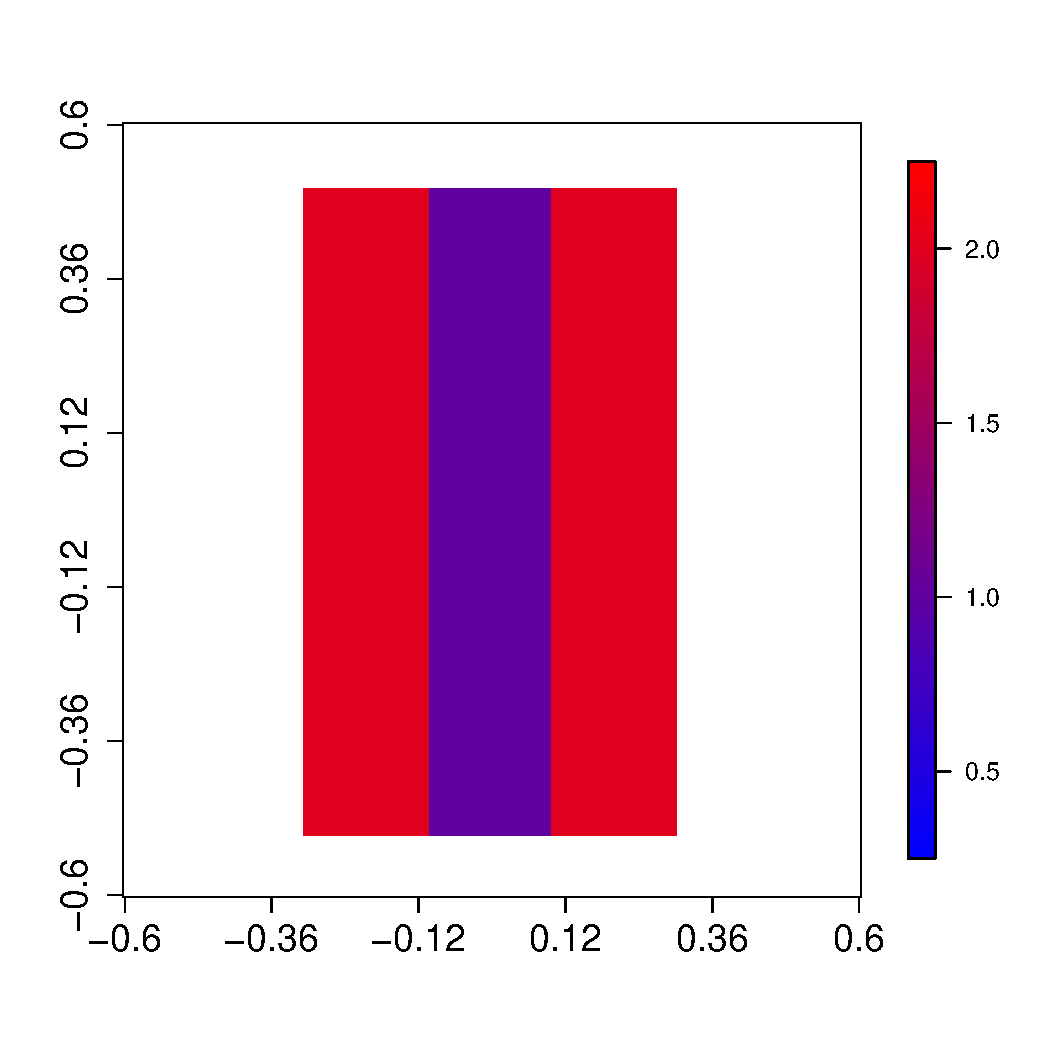
\includegraphics[width=0.495\textwidth]{../lower_bound_1}
	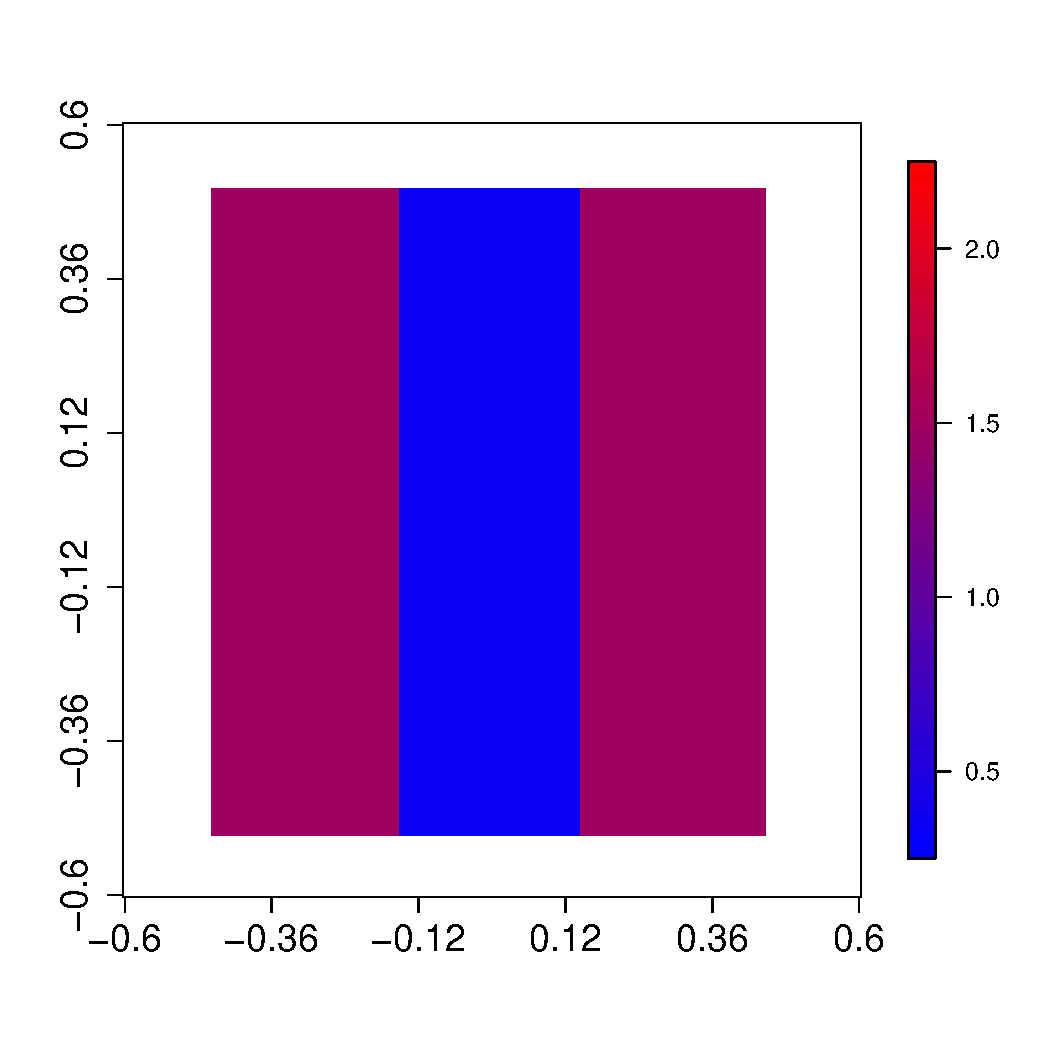
\includegraphics[width=0.495\textwidth]{../lower_bound_2}
	\caption{\it\small The density $f$ in \eqref{eqn:lb_density}, for
		$\rho=1$, and two different choices of $\epsilon$ and $\sigma$. Left:
		$\epsilon = 0.3$ and $\sigma = 0.1$; right: $\epsilon = 0.2$ and 
		$\sigma = 0.2$.} 
	\label{fig:hard_case}
\end{figure}

\paragraph{Lower bound on symmetric set difference.}

As the following theorem demonstrates, even when Algorithm~\ref{alg:ppr} is
reasonably initialized, if the density cluster \smash{$\mc{C}^{(1)}$} is 
sufficiently geometrically ill-conditioned (in words, tall and thin) the cluster 
estimator $\wh{C}$ will fail to recover \smash{$\mc{C}^{(1)}$}. Let
\begin{equation}
\label{eqn:lower_set}
\mathcal{L} = \set{(x_1,x_2) \in \mathcal{X}: x_2 < 0}.
\end{equation}

\begin{theorem}
	\label{thm:ppr_lb}
	Assume the radius $r < \min\set{\frac{1}{40}\rho, \frac{1}{4}\sigma}$, and that Algorithm~\ref{alg:ppr} is initialized using inputs $\alpha = 65  
	\Phi_{\Pbb,r}(\mathcal{L})$, and $(L,U) = (0,1)$.  Then, for any 
	\begin{equation*}
	n \geq \max\set{\frac{64}{\epsilon^2 \rho \sigma \pi r^2},
		\frac{8}{\epsilon}}, 
	\end{equation*}
	the following statement holds with probability at least $1 - B_3 n \exp\set{-b_3 n}$: there exists a set $\mc{C}[X]^g$ of large volume, \smash{$\vol_{n,r}(\mc{C}[X]^g \cap 
		\mc{C}^{(1)}[X]) \geq \vol_{n,r}(\mc{C}^{(1)}[X];G_{n,r})/10$}, such
	that for any seed node $v \in \mc{C}[X]^g$, the PPR estimated cluster
	\smash{$\wh{C}$} satisfies    
	\begin{equation}
	\label{eqn:ppr_lb}
	\frac{\sigma \rho}{r^2 n^2} \cdot \vol_{n,r}(\wh{C} \vartriangle
	\mc{C}^{(1)}[X]) \geq \frac{1}{4} -  C_4 \cdot 
	\frac{\sqrt{\sigma/\rho}}{\epsilon^2} \cdot \sqrt{ \log\left(\frac{\rho \sigma}
		{\epsilon^2 r^2}\right) \frac{\sigma}{r}},   
	\end{equation}
	Consequently, if
	\begin{equation*}
	\epsilon^2 \geq \frac{C_4}{8} \cdot \sqrt{\frac{\sigma}{\rho}} \cdot \sqrt{ 
		\log\left(\frac{\rho \sigma}{\epsilon^2 r^2}\right)\frac{\sigma}{r}}, 
	\end{equation*}
	then with high probability \smash{$\frac{\sigma
			\rho}{r^2 n^2} \cdot \vol_{n,r}(\wh{C} \vartriangle \mc{C}^{(1)}[X]) 
		\geq 1/8$}.    
\end{theorem}

%Note that for large enough $n$, $\vol_{n,r}(\mc{C}^{(1)}[X])$  will be close to $n^2 r^2/(\sigma\rho)$, and therefore the quantity \smash{$\frac{\sigma \rho}{r^2 n^2} \cdot \vol_{n,r}(\wh{C} \vartriangle \mc{C}^{(1)}[X])$} in \eqref{eqn:ppr_lb} is comparable to \smash{$\vol_{n,r}(\wh{C} \vartriangle \mc{C}^{(1)}[X]) / \vol_{n,r}(\mc{C}^{(1)}[X])$}, which corresponds to the quantity we upper bound in Corollary~\ref{thm:volume_ssd_ub}.   

Theorem~\ref{thm:ppr_lb} is stated with respect to a particular hard case, where
the density clusters are rectangular subsets of $\Reals^2$.  We chose this
setting to make the theorem simple to state, and our results are generalizable
to $\Reals^d$ and to non-rectangular clusters.  Moreover, although we state
our lower bound with respect to PPR run on a neighborhood graph, the conclusion is
likely to hold for a much broader class of spectral clustering algorithms. In
the proof of Theorem~\ref{thm:ppr_lb}, we rely heavily on the fact that when
$\epsilon^2$ is sufficiently greater than $\sigma/\rho$, the normalized cut of
$\mc{C}^{(1)}$ will be much larger than that of $\mathcal{L}$. In this case, not
merely PPR but any algorithm that approximates the minimum normalized cut is
unlikely to recover $\mc{C}^{(1)}$. In particular, local spectral clustering
algorithms based on truncated random walks \citep{spielman2013}, global spectral
clustering algorithms \citep{shi00}, and $p$-Laplacian based spectral embeddings
\citep{hein2010} all have provable upper bounds on the normalized cut of cluster
they output, and thus we expect that they would all fail to estimate
$\mc{C}^{(1)}$.

\paragraph{Comparison between upper and lower bounds.}

To better digest the implications of Theorem~\ref{thm:ppr_lb}, we translate the
results of our upper bound in Corollary~\ref{cor:density_cluster_volume_ssd_ub} to the density $f$ given in \eqref{eqn:lb_density}. Observe that $\mc{C}^{(1)}$ satisfies each of the Assumptions~\ref{asmp:lambda_bounded_density}--\ref{asmp:bounded_volume}:

\begin{enumerate}[label=(A\arabic*)]
	\item The density $f(x) = \frac{1 - \epsilon}{2 \rho \sigma}$ for all $x \in
	\mc{C}^{(1)}$.  
	\item The density $f(x) = \frac{\epsilon}{\rho\sigma}$ for all $x$ such
	that $0 < \dist(x,\mc{C}^{(1)}) \leq \sigma$. Therefore for all such $x$, 
	$$
	\inf_{x' \in \mc{C}^{(1)}} f(x') - f(x)  = \left\{\frac{1 - \epsilon}{2} -
	\epsilon \right\} \frac{1}{\rho \sigma},
	$$
	which meets the decay requirement with exponent $\gamma=0$.
	\item The set $\mc{C}^{(1)}$ is itself convex, and has diameter $\rho$.
	\item By symmetry, \smash{$\vol_{\Pbb,r}(\mc{C}^{(1)}) =
		\vol_{\Pbb,r}(\mc{C}^{(2)})$}, and therefore
	\smash{$\vol_{\Pbb,r}(\mc{C}^{(1)}) \leq \frac{1}{2}\vol_{\Pbb,r}(\Reals^d)$}.   
\end{enumerate}

\begin{remark}
	Technically, the rectangles $\mc{C}^{(0)},\mc{C}^{(1)},\mc{C}^{(2)}$ are not
	$\sigma$-expansions due to their sharp corners. To fix this, one can   
	%either modify the upper bound (specifically, Lemma~\ref{lem: expansion_volume}
	%in the proof of Theorem~\ref{thm: conductance_upper_bound}) to hold with
	%respect to rectangles of width $\sigma$, or  
	simply modify these sets to have appropriately rounded corners, and our lower
	bound arguments do not need to change significantly, subject to some
	additional bookkeeping.  Thus we ignore this technicality in our subsequent
	discussion. 
\end{remark}

If the user-specified parameters are initialized according to~\eqref{eqn:initialization}, we may apply Corollary~\ref{cor:density_cluster_volume_ssd_ub}. This implies that 
there exists a set $\mc{C}^{(1)}[X] \subseteq \mc{C}^{(1)}$ with
\smash{$\vol_{n,r}(\mc{C}[X]^g) \geq \frac{1}{2}\vol_{n,r}(\mc{C}[X])$} such
that for any seed node $v \in \mc{C}^{(1)}[X]$, and for large enough $n$, the
PPR estimated cluster $\wh{C}$ satisfies with high probability
\begin{equation*}
\frac{\vol_{n,r}(\wh{C} \vartriangle \mc{C}^{(1)}[X])}{\vol_{n,r}(\mc{C}^{(1)}[X])} \leq 64 C_{1,\delta} \cdot \frac{\rho^2}{\sigma r} \cdot \frac{\epsilon}{1 - \epsilon} \cdot \log^2\biggl(\sqrt{C_{2,\delta}} \frac{\rho}{r}\biggr)
\end{equation*}
To facilitate comparisons between our upper
and lower bounds, assume $\sigma/4 \leq \rho/40$ and set $r = \sigma/8$.  Then
the following statements each hold with high probability. 
\begin{itemize}
	\item If the user-specified parameters satisfy~\eqref{eqn:initialization}, and
	\begin{equation*}
	\frac{\epsilon}{1 - \epsilon} \leq \frac{a}{64C_{1,\delta}} \left(\frac{\sigma}{\rho \log(\rho/\sigma \sqrt{C_{2,\delta}})}\right)^2,
	\end{equation*}
	then \smash{$\Delta(\wh{C}, \mc{C}^{(1)}[X]) \leq a \cdot
		\vol_{n,r}(\mc{C}^{(1)}[X])$}.
	
	\item If the user-specified parameters are as in Theorem~\ref{thm:ppr_lb}, and
	\begin{equation*}
	\epsilon \geq \sqrt{\frac{C_4}{8}} \left({\frac{\sigma}{\rho}} \log^2 \left(\frac{\rho}
	{\epsilon^2 \sigma}\right)\right)^{1/4},
	\end{equation*}
	then \smash{$\Delta(\wh{C}, \mc{C}^{(1)}[X]) \geq \frac{1}{8}
		\vol_{n,r}(\mc{C}^{(1)}[X])$}. 
\end{itemize}

Jointly, these upper and lower bounds give a relatively precise characterization
of what it means for a density cluster to be well- or poorly-conditioned for recovery using PPR. 

\begin{remark}
	It is worth pointing out that the above conclusions are reliant on specific
	(albeit reasonable) ranges and choices of input parameters, which in some
	instances differ between the upper and lower bounds. We suspect that our lower
	bound continues to hold even when choosing input parameters as dictated by our
	upper bound, but do not pursue the details.
\end{remark}

Finally, it is not hard to show that in the example under consideration, classical
plug-in density cluster estimators can consistently recover the
$\sigma$-expansion $\mc{C}_{\lambda,\sigma}$ of a density cluster $\mc{C}_{\lambda}$, even if $\epsilon$ is
large compared to $\sigma/\rho$. That PPR has trouble recovering density
clusters here (where standard plug-in approaches do not) is not meant to
be a knock on PPR. Rather, it simply reflects that while classical density
clustering approaches are specifically designed to identify high-density regions
regardless of their geometry, PPR relies on geometry as well as density when
forming the output cluster. 

\section{Experiments}
\label{sec:experiments}

We provide numerical experiments to investigate the tightness of our theoretical results, and examine the performance of PPR on the ``two moons'' dataset. We defer details of the experimental settings to the appendix.   

\begin{figure}[tb]
	\centering
	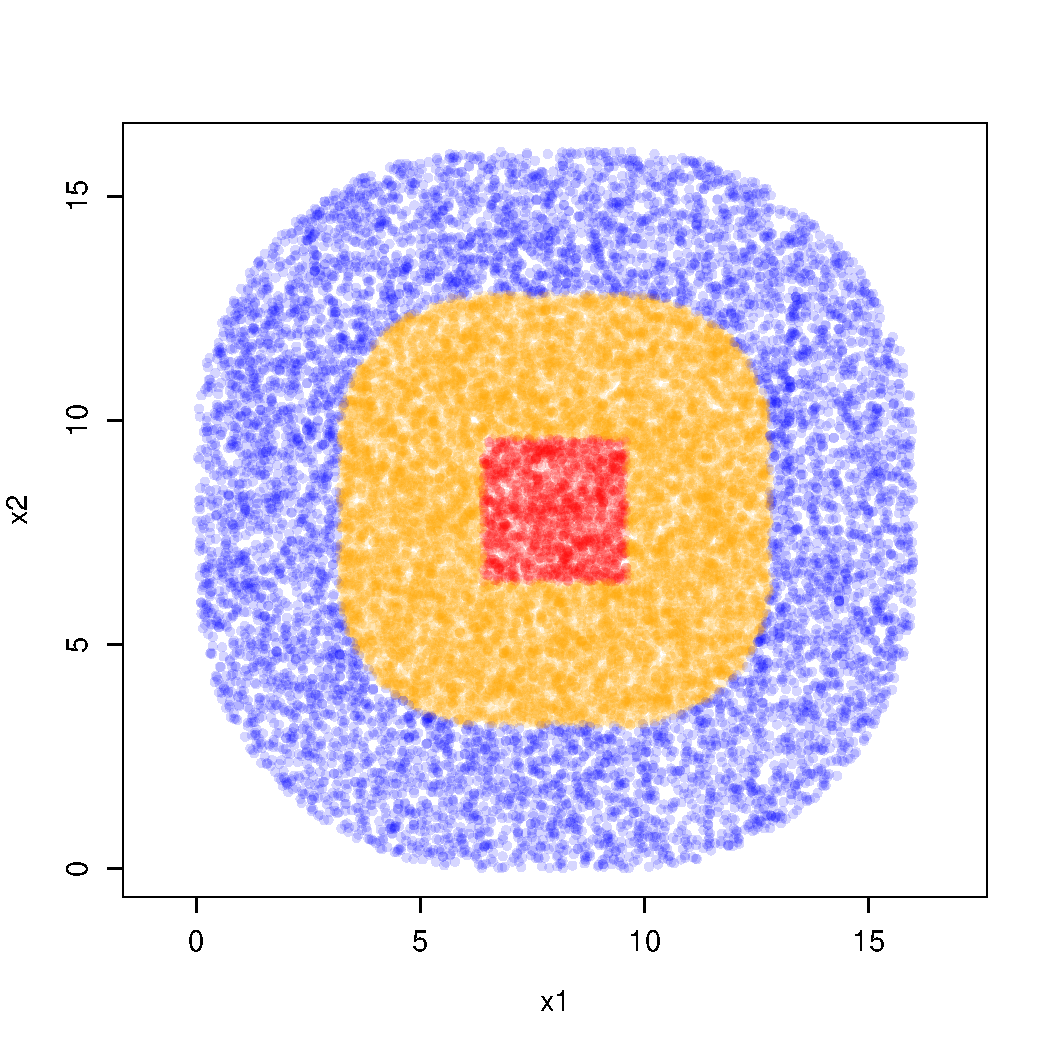
\includegraphics[width=0.32\textwidth]{../sample2}
	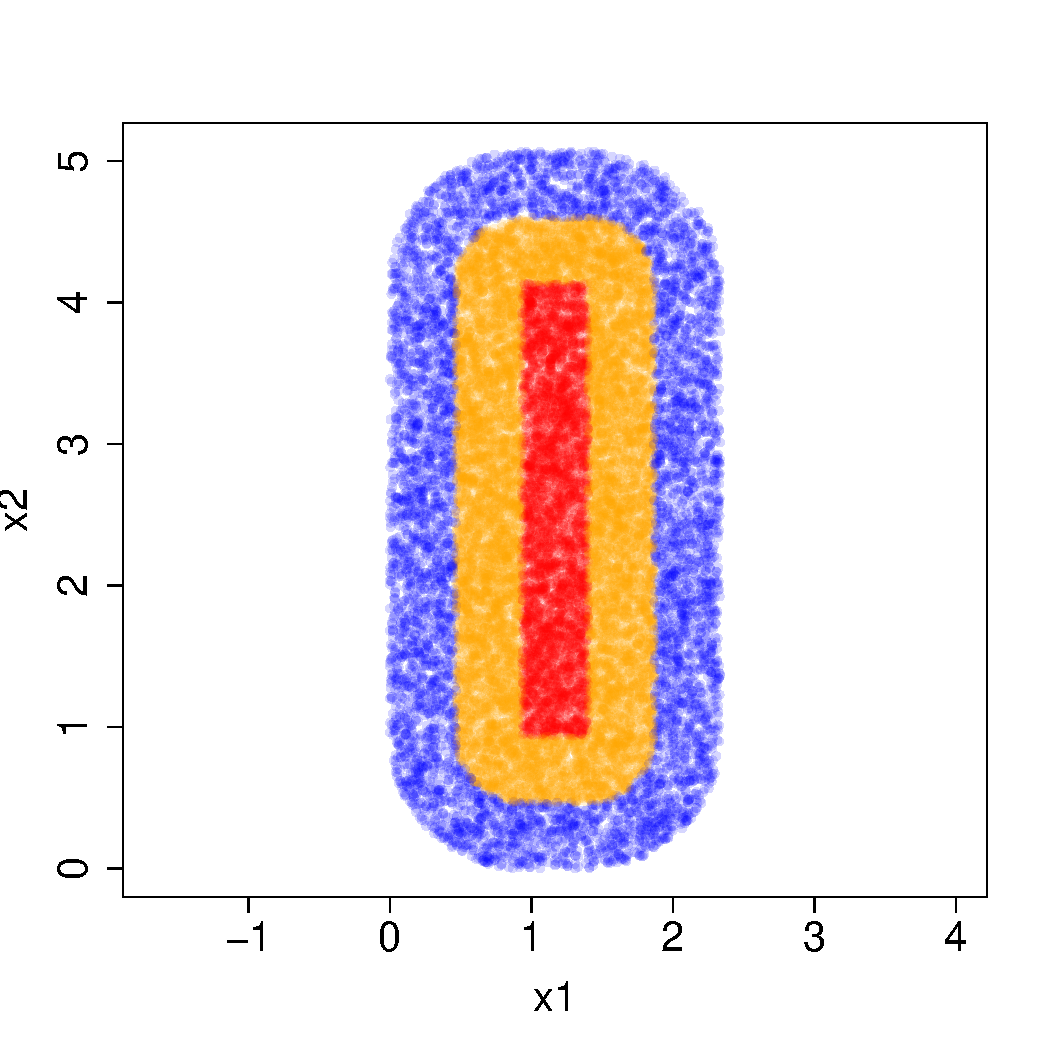
\includegraphics[width=0.32\textwidth]{../sample1}
	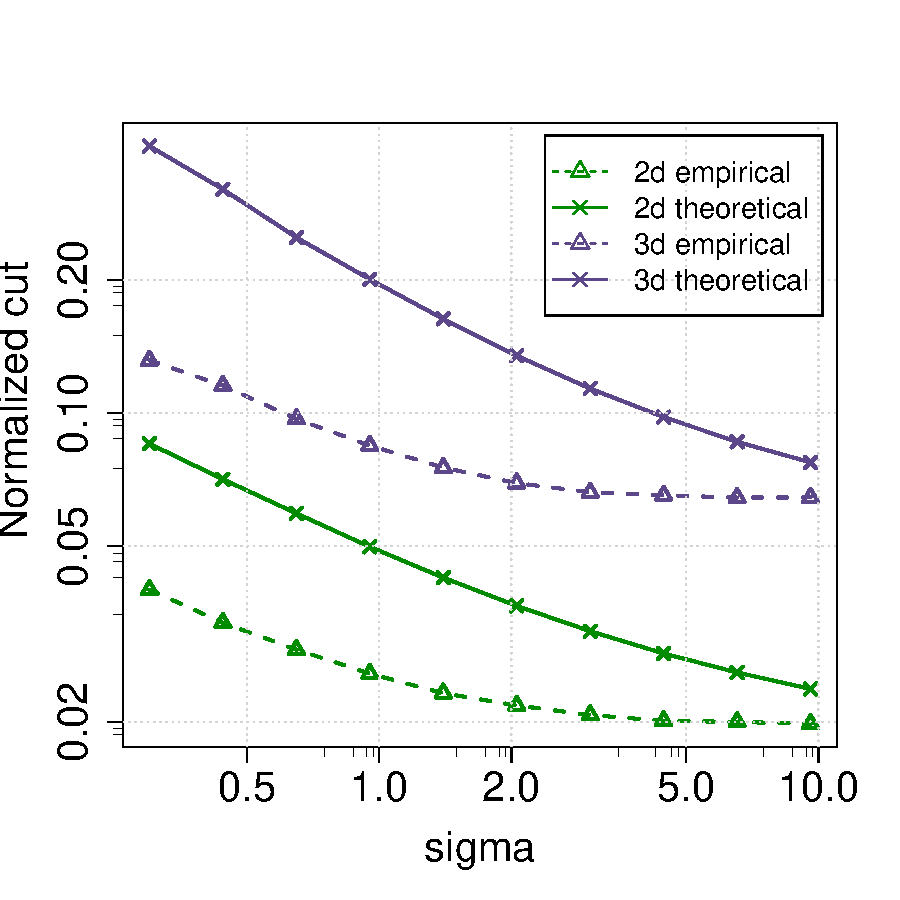
\includegraphics[width=0.32\textwidth]{../sigma_normalized_cut_plot}
	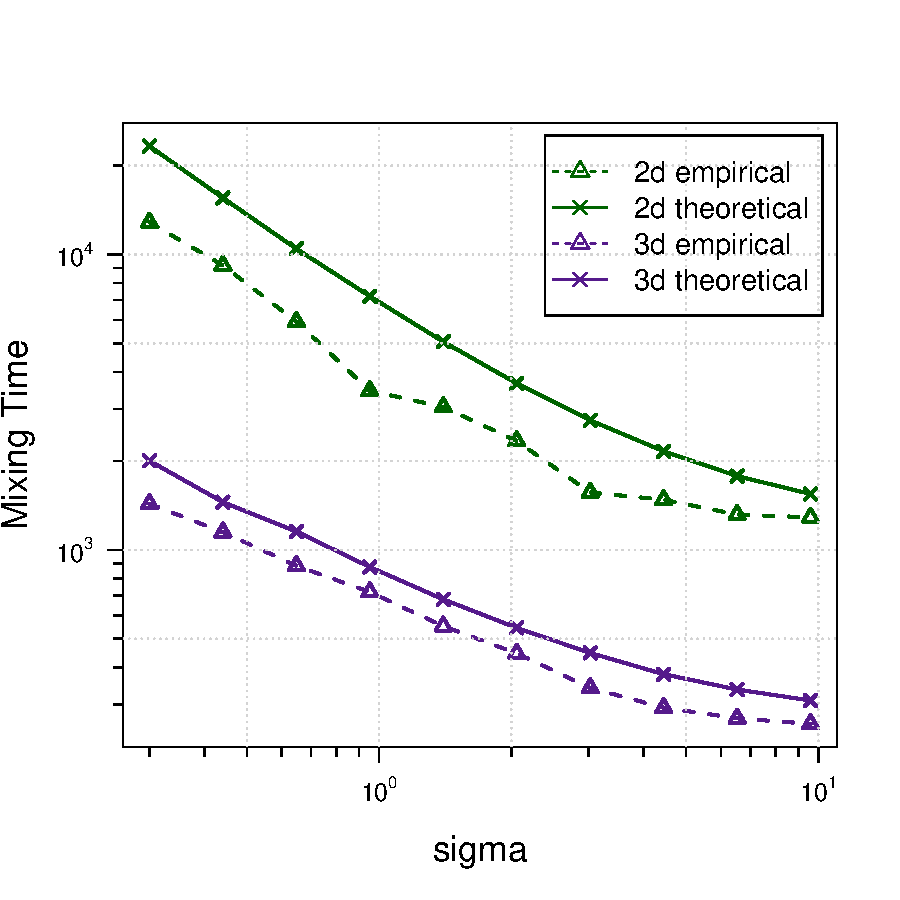
\includegraphics[width=0.32\textwidth]{../sigma_mixing_time_plot}
	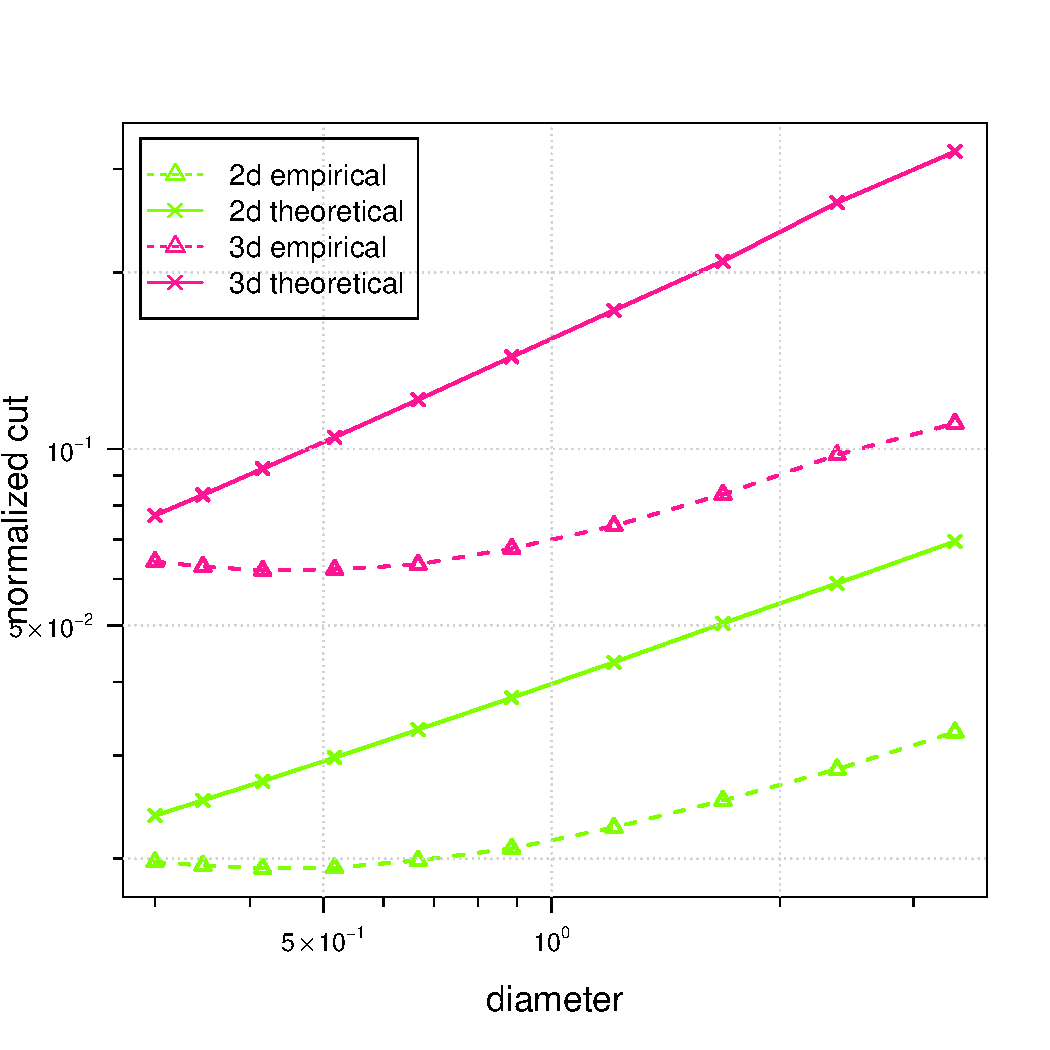
\includegraphics[width=0.32\textwidth]{../diameter_normalized_cut_plot}
	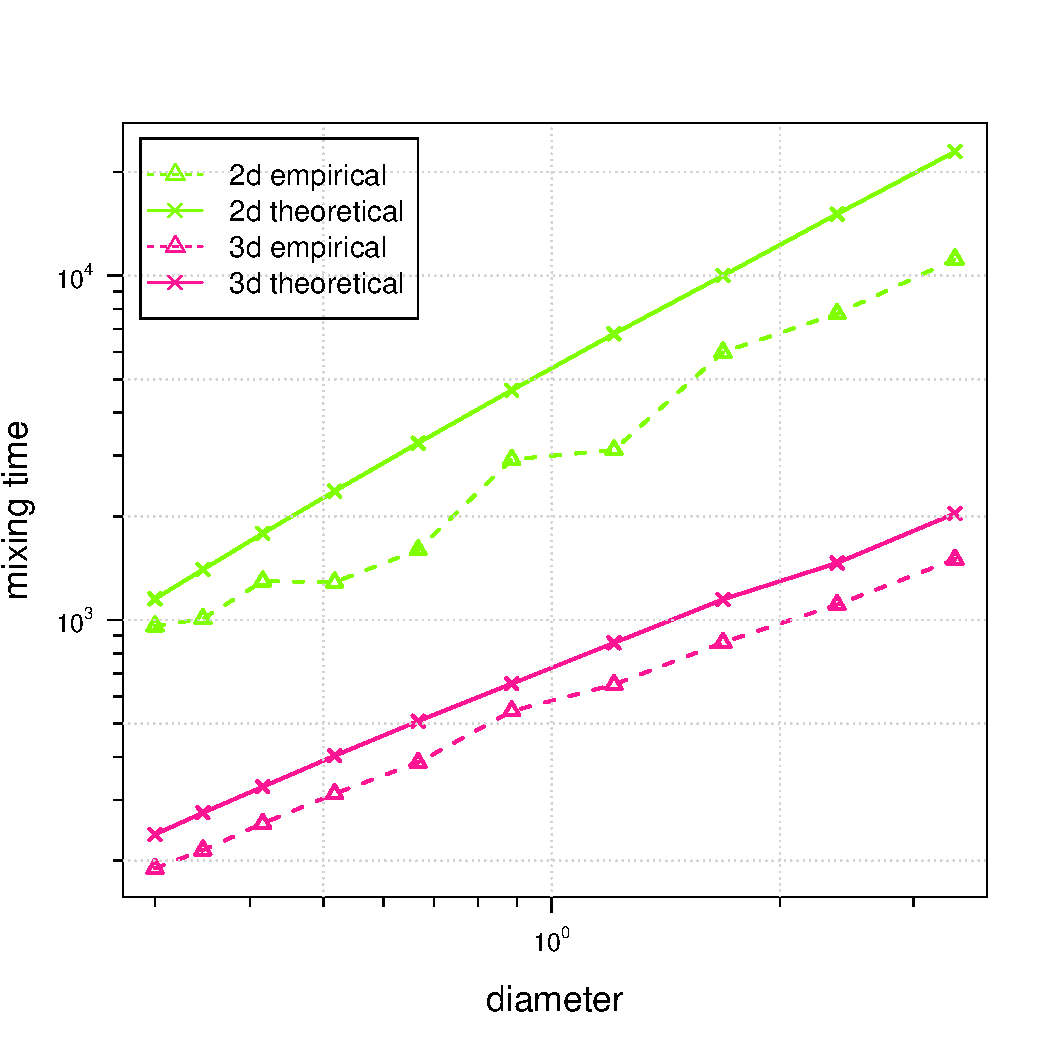
\includegraphics[width=0.32\textwidth]{../diameter_mixing_time_plot}
	\caption{\it\small Top left and top middle: samples from a geometrically
		well- and poor-conditioned cluster. The points in $\mc{C}_{\lambda}$ are colored in red, points in $\mc{C}_{\lambda,\sigma} \!\setminus\! \mc{C}_{\lambda}$ are colored in yellow, and the remaining points in blue. Other panels: empirical normalized cut and mixing time, as a function of $\sigma$ or $\rho$, versus their theoretical upper bounds.} 
	\label{fig:bounds}
\end{figure}

\paragraph{Validating theoretical bounds.}  We investigate the tightness of
Propositions~\ref{prop:density_cluster_normalized_cut} and Proposition~\ref{prop:density_cluster_conductance}, as well as the resulting Corollary~\ref{cor:density_cluster_volume_ssd_ub}, via simulation. Figure \ref{fig:bounds} compares our bounds on normalized cut and conductance with the actual empirically-computed quantities \eqref{eqn:normalized_cut} and \eqref{eqn:conductance}, as we vary the diameter $\rho$ and thickness $\sigma$ of a cluster $\mc{C}$. The top left and top middle panels display the resulting empirical clusters for two different values of $\rho,\sigma$. 

The bottom left and bottom right panels assure that our lower bounds on conductance track closely with the empirical conductance, in both 2 and 3 
dimensions.\footnote{We rescaled all values of theoretical bounds by a constant, to mask the effect of large universal constants in these bounds. Therefore only the comparison of slopes, rather than intercepts, is meaningful.} \textcolor{red}{(TODO): Need to change the ``mixing time'' panels to ``conductance'' panels.} This provides empirical evidence that Proposition~\ref{prop:density_cluster_conductance} has the right dependency on both expansion parameter $\sigma$ and diameter $\rho$. The story for the normalized cut panels
is less obvious. We remark that while, broadly speaking, the trends do not
appear to match, this gap between theory and empirical results seems largest
when $\sigma $ and $\rho$ are approximately equal. As the ratio $\rho/\sigma$
grows, the slopes of empirical and theoretical curves become more similar.

\textcolor{red}{(TODO): Include a second figure comparing the volume of the symmetric set difference with our upper bound on the volume of the symmetric set difference. Point out that this comparison also validates Theorem~\ref{thm:volume_ssd_ub}, since Corollary~\ref{cor:density_cluster_volume_ssd_ub} is a corollary of this theorem.}

\paragraph{Empirical behavior of PPR.} In Figure \ref{fig:moons}, to drive home 
the implications of Section~\ref{sec:ppr_density_cluster}, we show the behavior of PPR,
normalized cut, and the density clustering algorithm of \citet{chaudhuri2010} on
the well-known ``two moons'' dataset (with added 2d Gaussian noise), considered
a prototypical success story for spectral clustering algorithms. The first
column shows the empirical density clusters $\mc{C}[X]$ and $\mc{C}'[X]$ for
a particular threshold $\lambda$ of the density function; the second column
shows the cluster recovered by PPR; the third column shows the global minimum
normalized cut, computed according to the algorithm of \citet{szlam2010}; and
the last column shows a cut of the density cluster tree estimator of
\citet{chaudhuri2010}.  We can see the degrading ability of PPR to recover
density clusters as the two moons become less well-separated. Of particular
interest is the fact that PPR fails to recover one of the moons even when
normalized cut still succeeds in doing so. Additionally, we note that the
Chaudhuri-Dasgupta algorithm succeeds even when both PPR and normalized cut
fail.  This supports our main message, which is that PPR recovers only
geometrically well-conditioned density clusters.

\begin{figure}
	\centering
	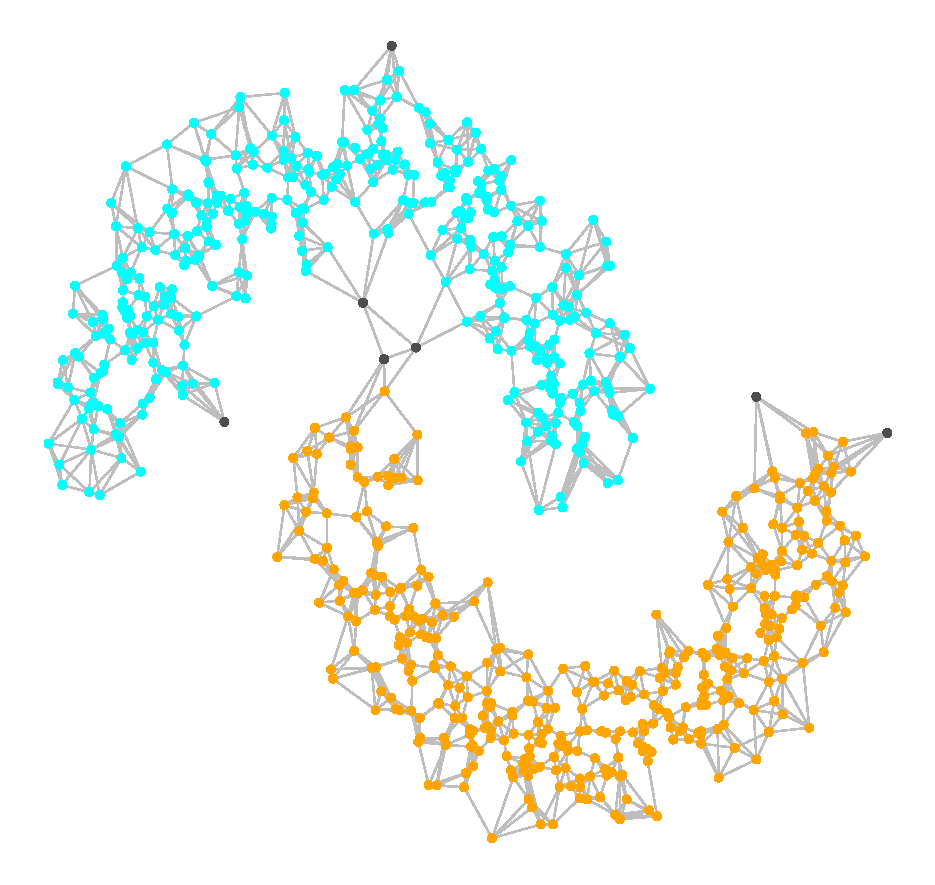
\includegraphics[width=0.24\textwidth,scale = .5]{../row1_true_density_cluster}
	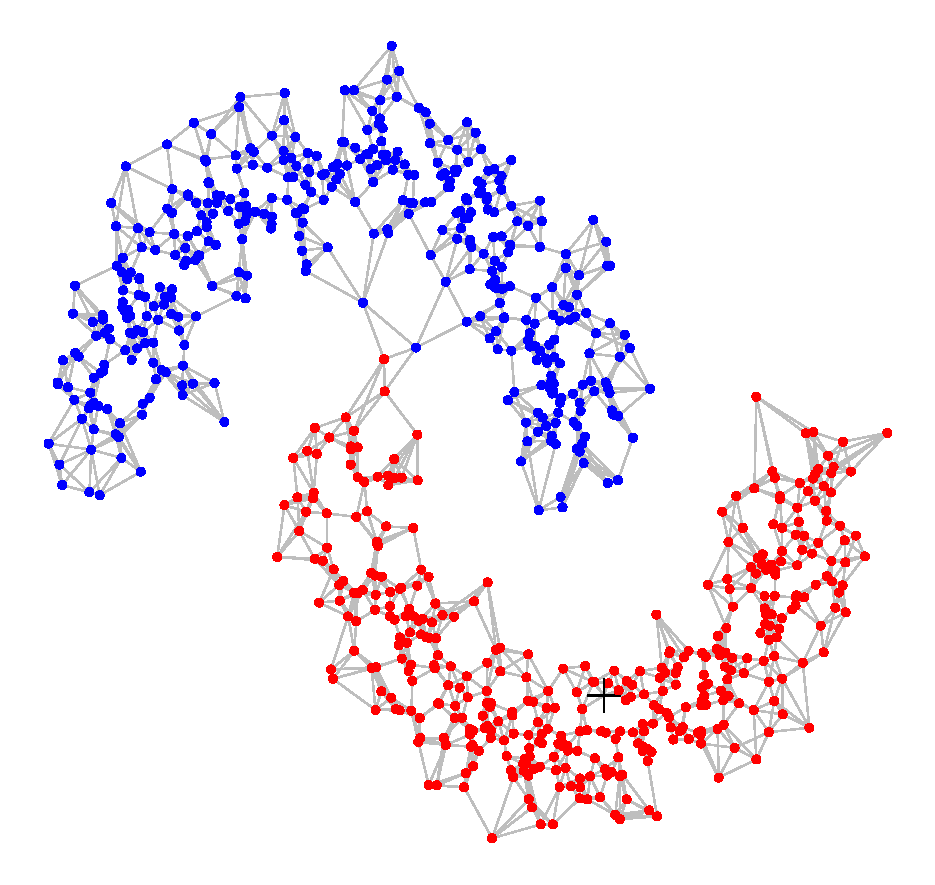
\includegraphics[width=0.24\textwidth]{../row1_ppr_cluster}
	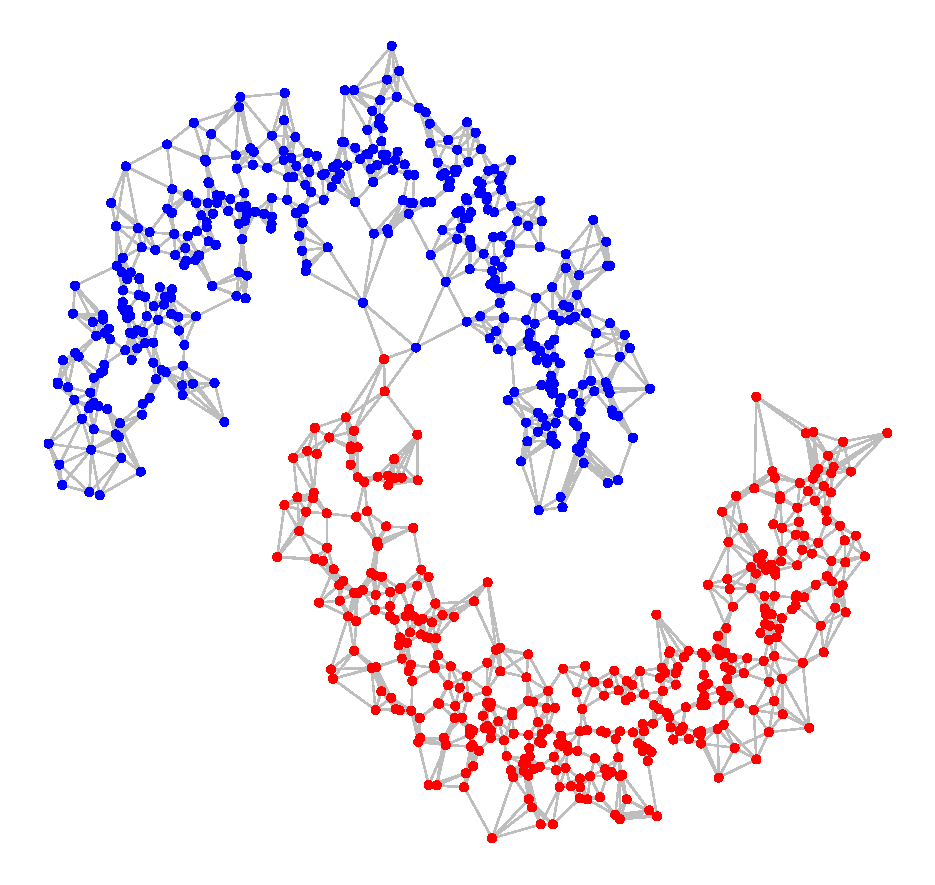
\includegraphics[width=0.24\textwidth]{../row1_conductance_cluster}
	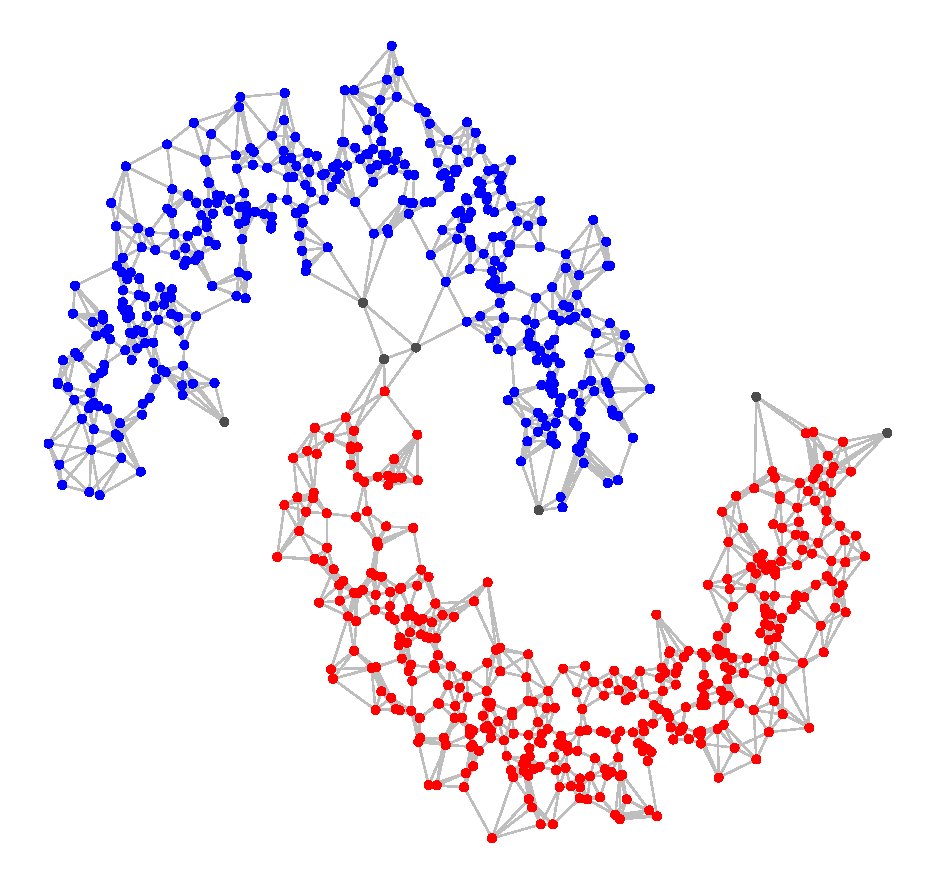
\includegraphics[width=0.24\textwidth]{../row1_density_cluster}
	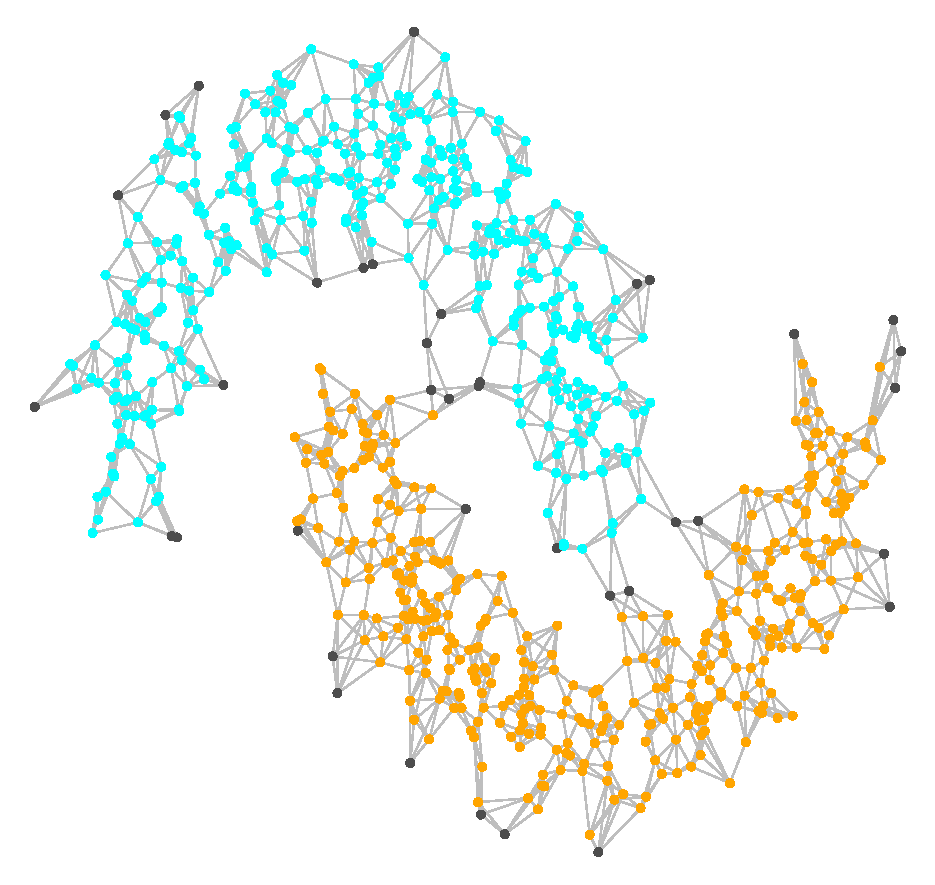
\includegraphics[width=0.24\textwidth]{../row2_true_density_cluster}
	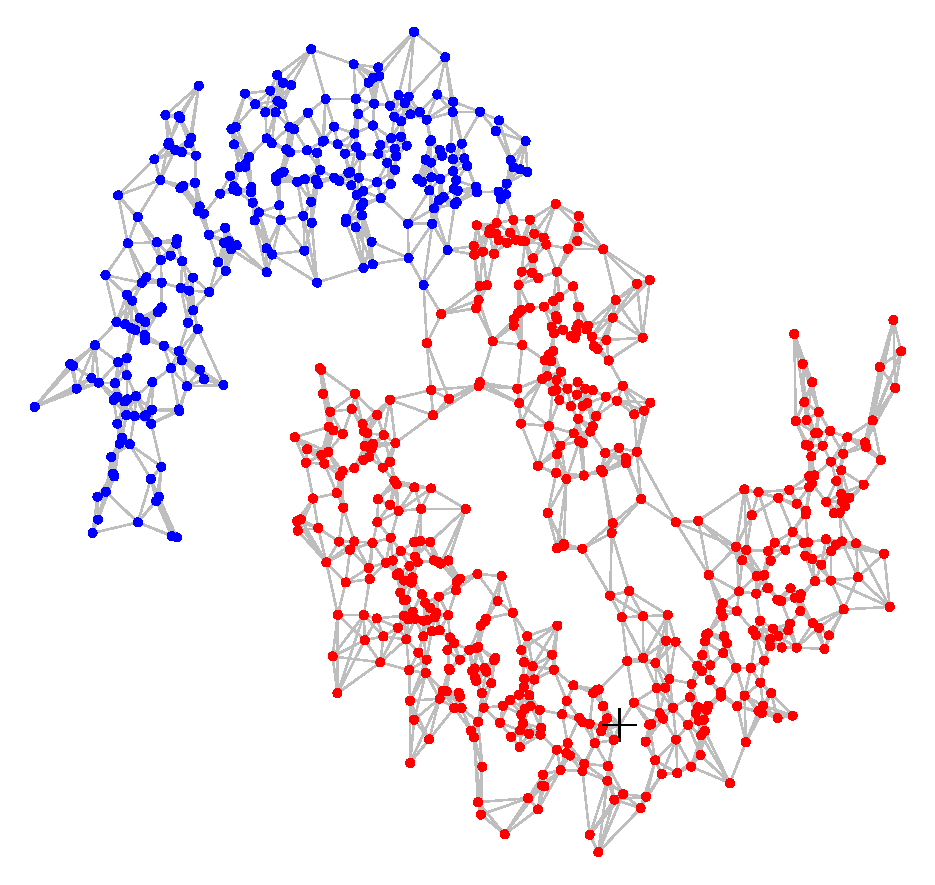
\includegraphics[width=0.24\textwidth]{../row2_ppr_cluster}
	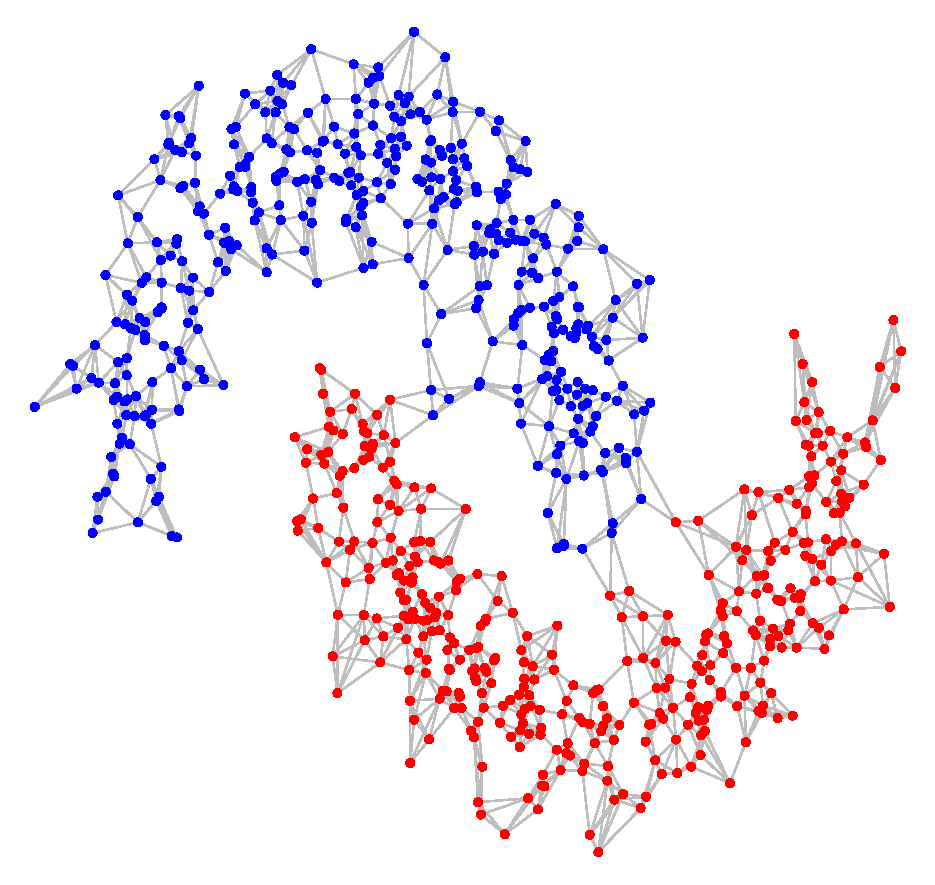
\includegraphics[width=0.24\textwidth]{../row2_conductance_cluster}
	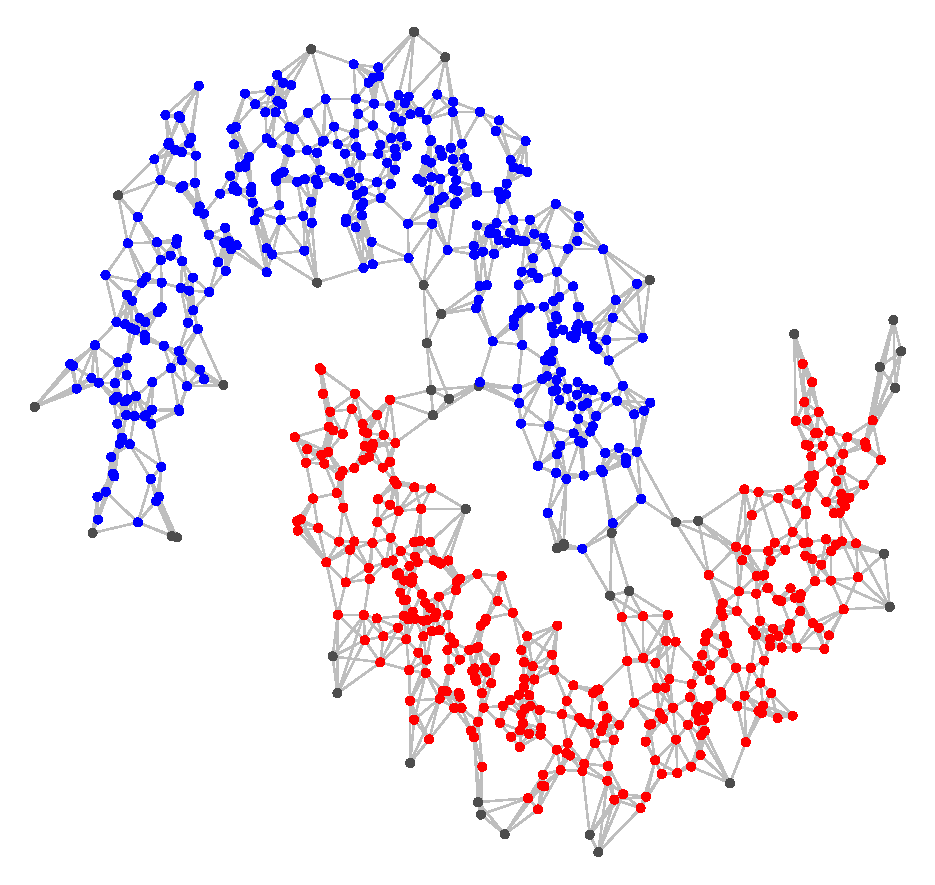
\includegraphics[width=0.24\textwidth]{../row2_density_cluster}
	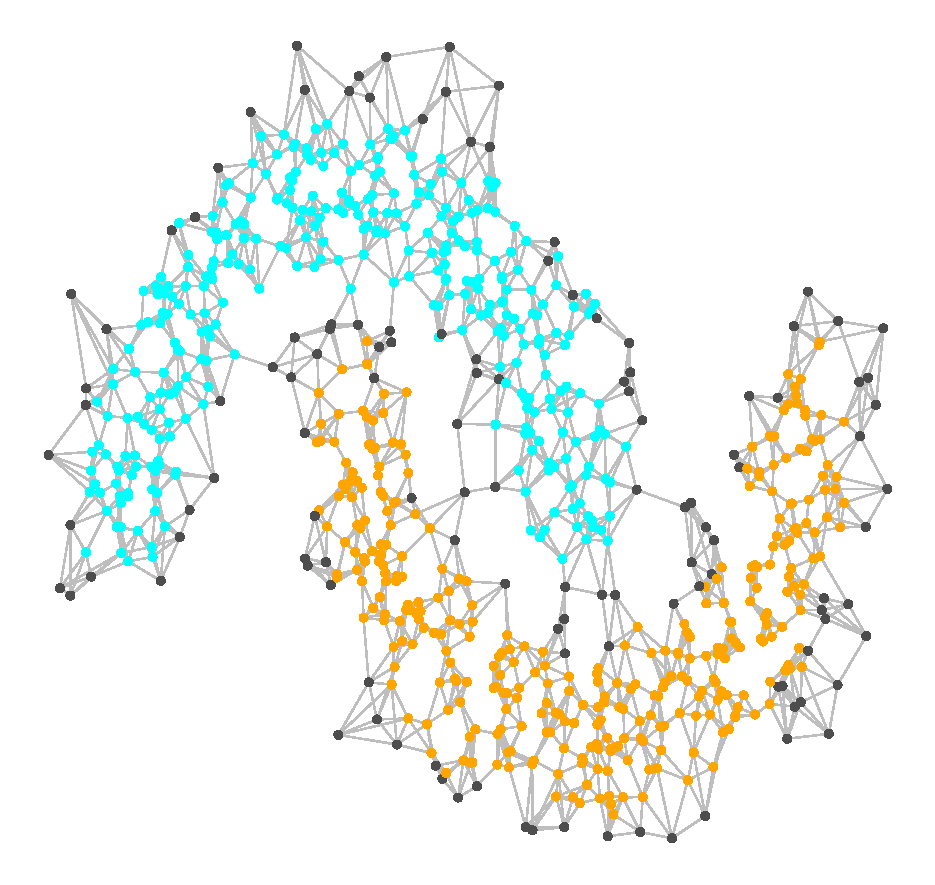
\includegraphics[width=0.24\textwidth]{../row3_true_density_cluster}
	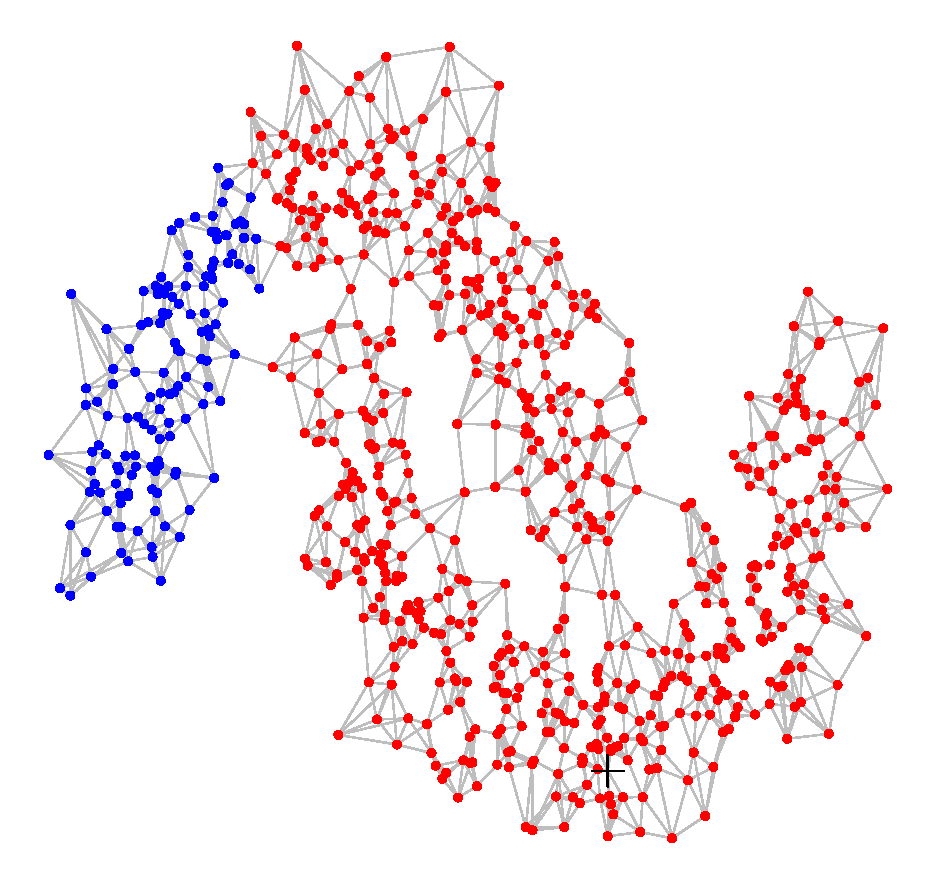
\includegraphics[width=0.24\textwidth]{../row3_ppr_cluster}
	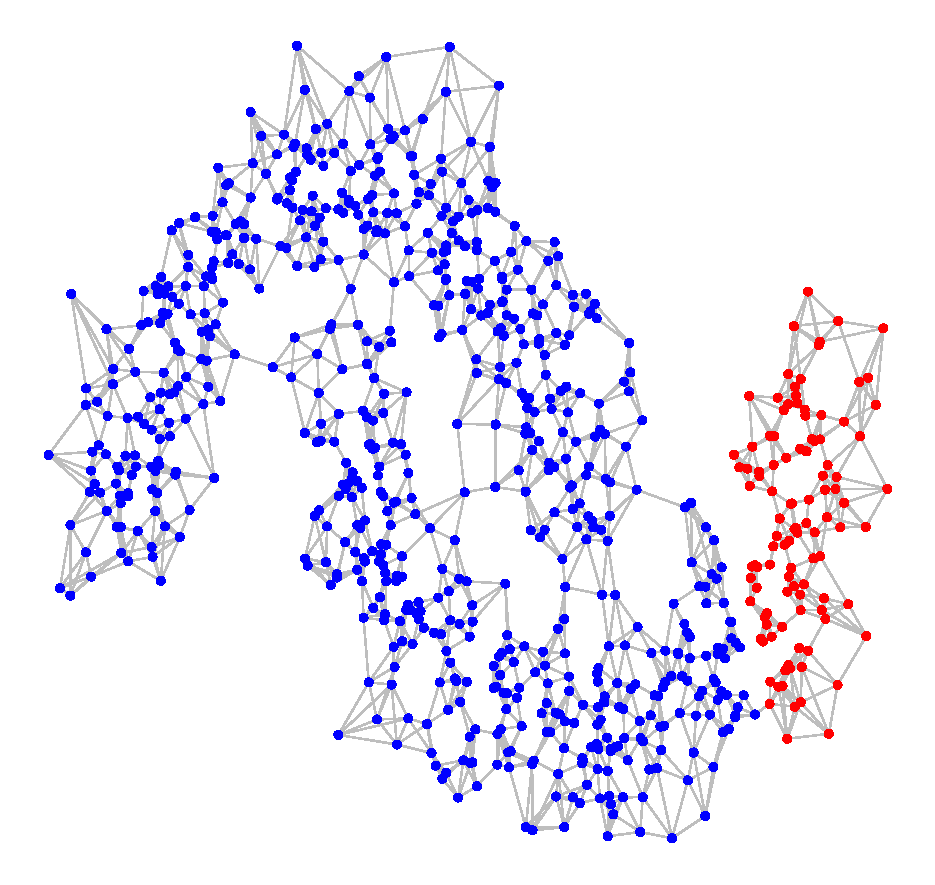
\includegraphics[width=0.24\textwidth]{../row3_conductance_cluster}
	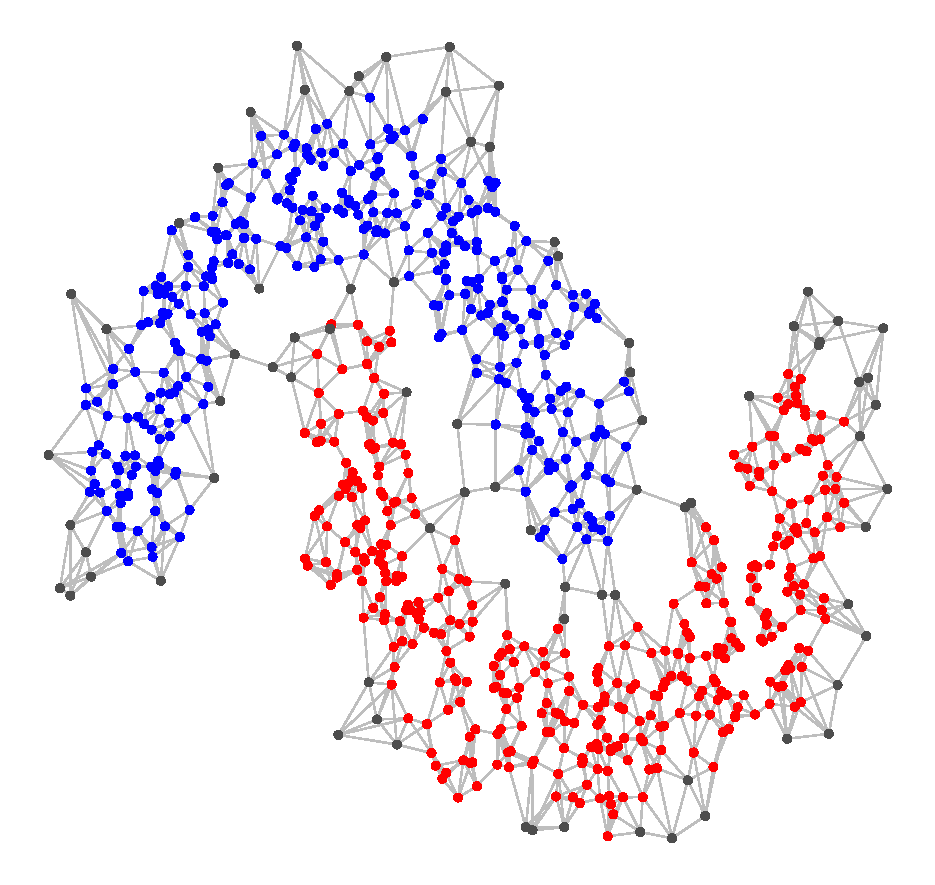
\includegraphics[width=0.24\textwidth]{../row3_density_cluster}
	\caption{\it\small True density (column 1), PPR (column 2), normalized
		cut (column 3) and estimated density (column 4) clusters for 3 different 
		simulated data sets. Seed node for PPR denoted by a black cross.} 
	\label{fig:moons}
\end{figure}


\section{Discussion}
\label{sec:discussion}
In this work, we have analyzed the behavior of PPR in the classical setup of non-parametric statistics. We have shown how PPR depends on the geometry of the distribution $\Pbb$ through the population level normalized cut, conductance, and local spread, and established upper bounds on the error with which PPR recovers an arbitrary candidate cluster $\mc{C} \subseteq \Rd$.  In the particularly important case where $\mc{C} = \mc{C}_{\lambda}$ is a $\lambda$-density cluster, we have shown that PPR recovers $\mc{C}_{\lambda}$ if and only if it is geometrically and vertically well-conditioned. We now conclude by summarizing several interesting directions for future work.

Letting the radius of the neighborhood graph shrink, $r \to 0$ as $n \to  
\infty$, would be computationally attractive, as it would ensure that the graph 
$G_{n,r}$ is sparse. However, the bounds~\eqref{eqn:volume_ssd_ub} and~\eqref{eqn:density_cluster_volume_ssd_ub} will blow up as the radius $r$ goes to $0$, preventing us from making claims about the behavior of PPR in
this regime. Although the restriction to a kernel function fixed in $n$ is
common in spectral clustering theory \citep{vonluxburg2008, schiebinger2015, singer2017},
recent works~\citep{shi2015, calder2019, garciatrillos18, garciatrillos2020, yuan2020} have demonstrated that spectral methods have meaningful continuum limits when $r \to 0$ as $n \to \infty$, and given precise rates of convergence.~\cite{garciatrillos19} have applied these results to analyze global spectral clustering in the nonparametric mixture model, obtaining asymptotic upper bounds that do not depend on $r$; it seems plausible that similar bounds could be obtained for local spectral clustering with PPR, although the arguments would necessarily be quite different.

In another direction, it would be very useful to find reasonable conditions under which the ratio $\Delta(\wh{C},\mc{C}[X])/\vol_{n,r}(\mc{C}[X])$ would tend to $0$ as $n \to \infty$. It seems likely that such a strong result would entail bounds on the $\Leb^{\infty}$-error of PPR (similar to~\eqref{eqn:ppr_gap}). Although most work thus far on spectral clustering methods has focused on deriving bounds on the $\Leb^1$- or $\Leb^2$-error, some recent works~\citep{dunson2020,calder2020} have established $\Leb^{\infty}$-bounds on the error with which the eigenvectors of a graph Laplacian matrix approximate the eigenvectors of a weighted Laplace-Beltrami operator. It is not clear whether the techniques used in these works can be applied to PPR.

Finally, after reading our Section~\ref{sec:ppr_density_cluster}, the practitioner may be tempted to ask why they should estimate a density cluster using PPR, when other methods are available with superior statistical guarantees. A rather prosaic, if undoubtedly correct, answer is that the ``ideal'' cluster is entirely in the eye of the beholder. For instance, it is quite common to define an ideal cluster as one with a small normalized cut, in which case the cluster output by PPR may be quite preferable to standard density clustering procedures. A more intriguing answer is that a (local) spectral method such as PPR may be more stable in the presence of noise than traditional density clustering procedures.\footnote{In the context of semi-supervised learning, a similar argument was alluded to by Misha Belkin and Partha Niyogi~\citep{belkin2002}, who say:
\begin{quote}
One possible simple approach is to use ``geodesic nearest neighbors''. However, while simple and well-motivated, this method is potentially unstable.	
\end{quote}
} Such a question could be answered by comparing the sample complexity of spectral clustering methods with density clustering procedures, but to our knowledge, the sample complexity of spectral methods remains unknown.

\section*{Acknowledgements}

SB is grateful to Peter Bickel, Martin Wainwright, and Larry Wasserman for
helpful and inspiring conversations. This work was supported in part by the NSF grant DMS-1713003.

\clearpage

\bibliography{../../local_spectral_bibliography} 

\end{document}